% LaTeX reconstruction of VHHreport.pdf
% paper-review-harbor: manuscript-pdf=VHHreport.pdf
% "Practical De Novo Nanobody Discovery with Tens of Experimental Candidates"
% MoleculeMind report (report format), June 2026.
% Faithful word-for-word reproduction of the PDF text; figures extracted from
% the PDF with pdfimages and embedded as PNGs beside this file.
\documentclass[11pt]{article}

\usepackage[letterpaper,margin=1in]{geometry}
\usepackage[T1]{fontenc}
\usepackage[utf8]{inputenc}
\usepackage{lmodern}
\usepackage{amsmath}
\usepackage{amssymb}
\usepackage{graphicx}
\usepackage{booktabs}
\usepackage{multirow}
\usepackage{textcomp}
\usepackage{fancyhdr}
\usepackage[colorlinks=true,linkcolor=blue,citecolor=blue,urlcolor=blue]{hyperref}

\pagestyle{fancy}
\fancyhf{}
\fancyhead[L]{MoleculeMind -- De Novo VHH Design Platform}
\fancyhead[R]{May 2026}
\fancyfoot[C]{\thepage}
\renewcommand{\headrulewidth}{0.4pt}
\setlength{\headheight}{14pt}

\begin{document}

\thispagestyle{empty}
\begin{center}
{\Large\bfseries Practical De Novo Nanobody Discovery\\[3pt] with Tens of Experimental Candidates}\\[14pt]
{\large Jinbo Xu on behalf of The MoleculeMind Team}\\[6pt]
correspondence to: \url{jinboxu@moleculemind.com}\\[4pt]
MoleuleMind Inc., Room 306, No. 1011 Halei Road, Pudong New District, Shanghai, China\\[6pt]
June 2026
\end{center}

\vspace{2ex}
\begin{center}\textbf{Abstract}\end{center}

Conventional antibody discovery relies on animal immunization or large-scale library screening,
requiring experimental interrogation of millions to billions of candidates with limited programmability over epitope specificity and molecular properties. Recent advances in generative
modeling have demonstrated the possibility of de novo antibody design, yet achieving experimentally practical biologics discovery at low experimental throughput across therapeutically
relevant targets remains challenging.

Here we present MMDesign, a de novo VHH discovery platform combining generative
sequence--structure optimization with multi-tier computational filtering. Starting from only
a target protein and specified epitope residues, MMDesign generates tens of thousands of
nanobody candidates through optimization over the confidence landscape of MMFold, a proprietary antibody--antigen structure prediction model, together with a protein language model.
Successive filtering stages incorporating structural reliability, sequence naturalness, and physicsbased interface evaluation compress the candidate pool to only tens of experimental testable
designs per target. We evaluated MMDesign across 11 therapeutically relevant targets spanning
cytokines, immune checkpoints, receptors, a viral protein, and a surface antigen. Experimental
testing of only 14--50 candidates per target yielded confirmed binders for 10 of 11 targets (90.9\%),
with best measured affinities ranging from picomolar to nanomolar levels, demonstrating broad
target-level success at experimentally tractable scale. Notably, MMDesign achieved a 50\% hit rate
on TNF$\alpha$, a shallow trimeric cytokine target that has proven difficult for prior low-throughput de
novo VHH discovery campaigns.

Together, these results suggest that biologics discovery may increasingly transition from largescale stochastic screening toward programmable molecular engineering, in which computational
generation and prioritization substantially reduce experimental burden while enabling rapid
epitope-targeted therapeutic binder discovery.

\section*{Graphical Abstract}
\begin{figure}[!htbp]
  \centering
  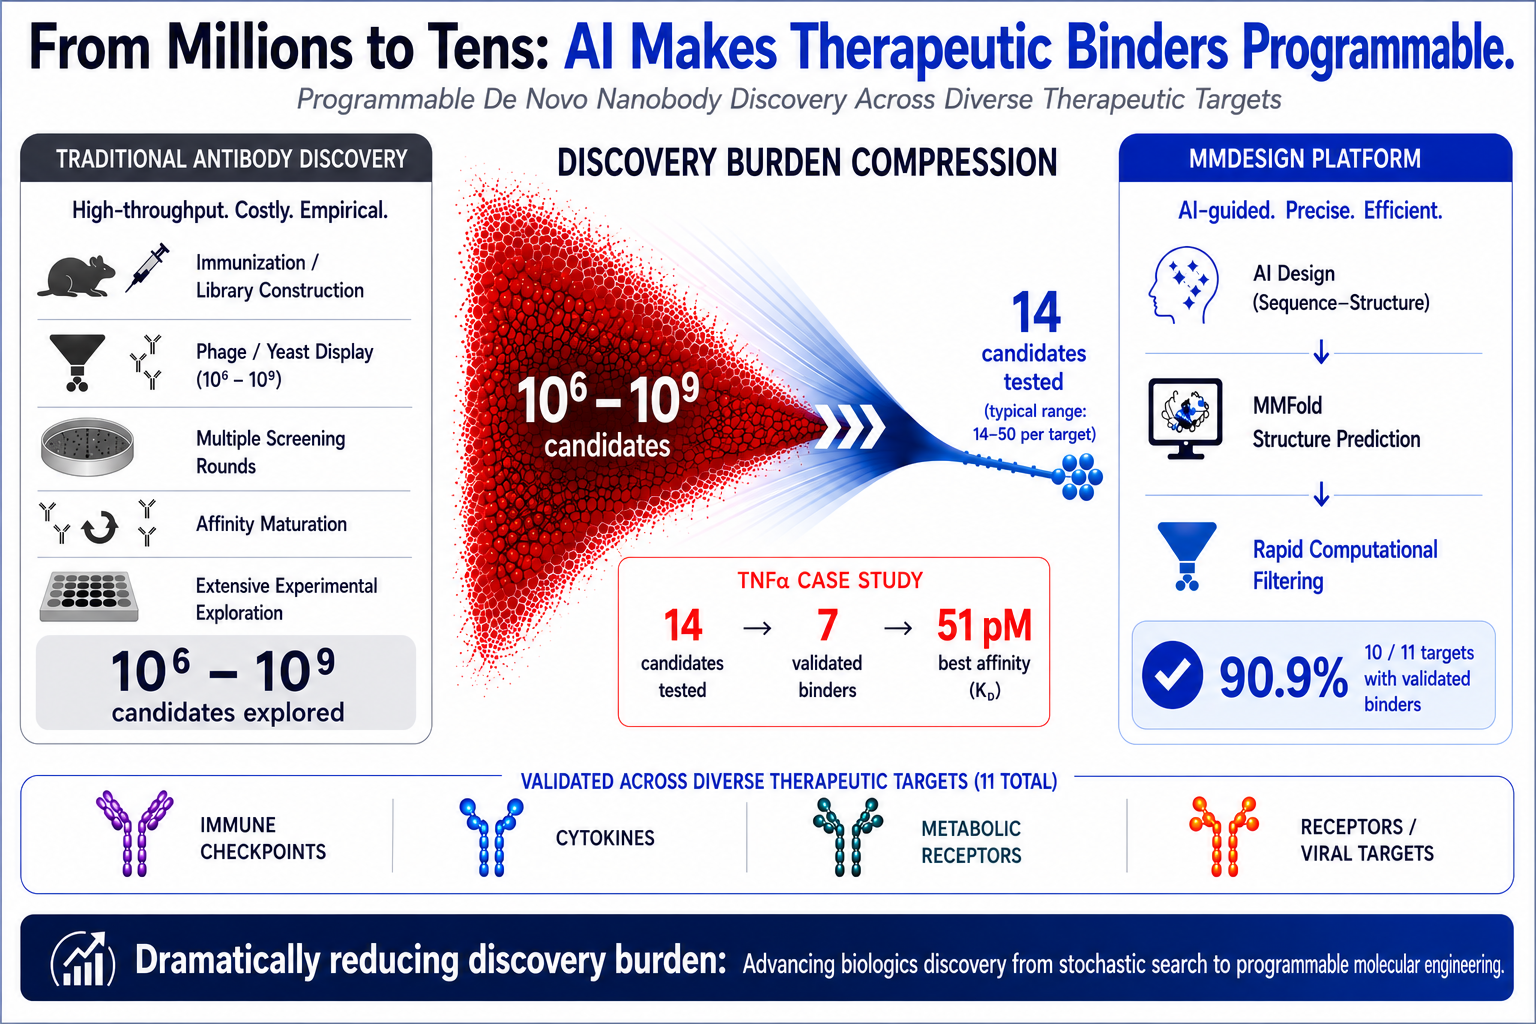
\includegraphics[width=\textwidth]{fig_abstract.png}
\end{figure}

\begin{figure}[!htbp]
  \centering
  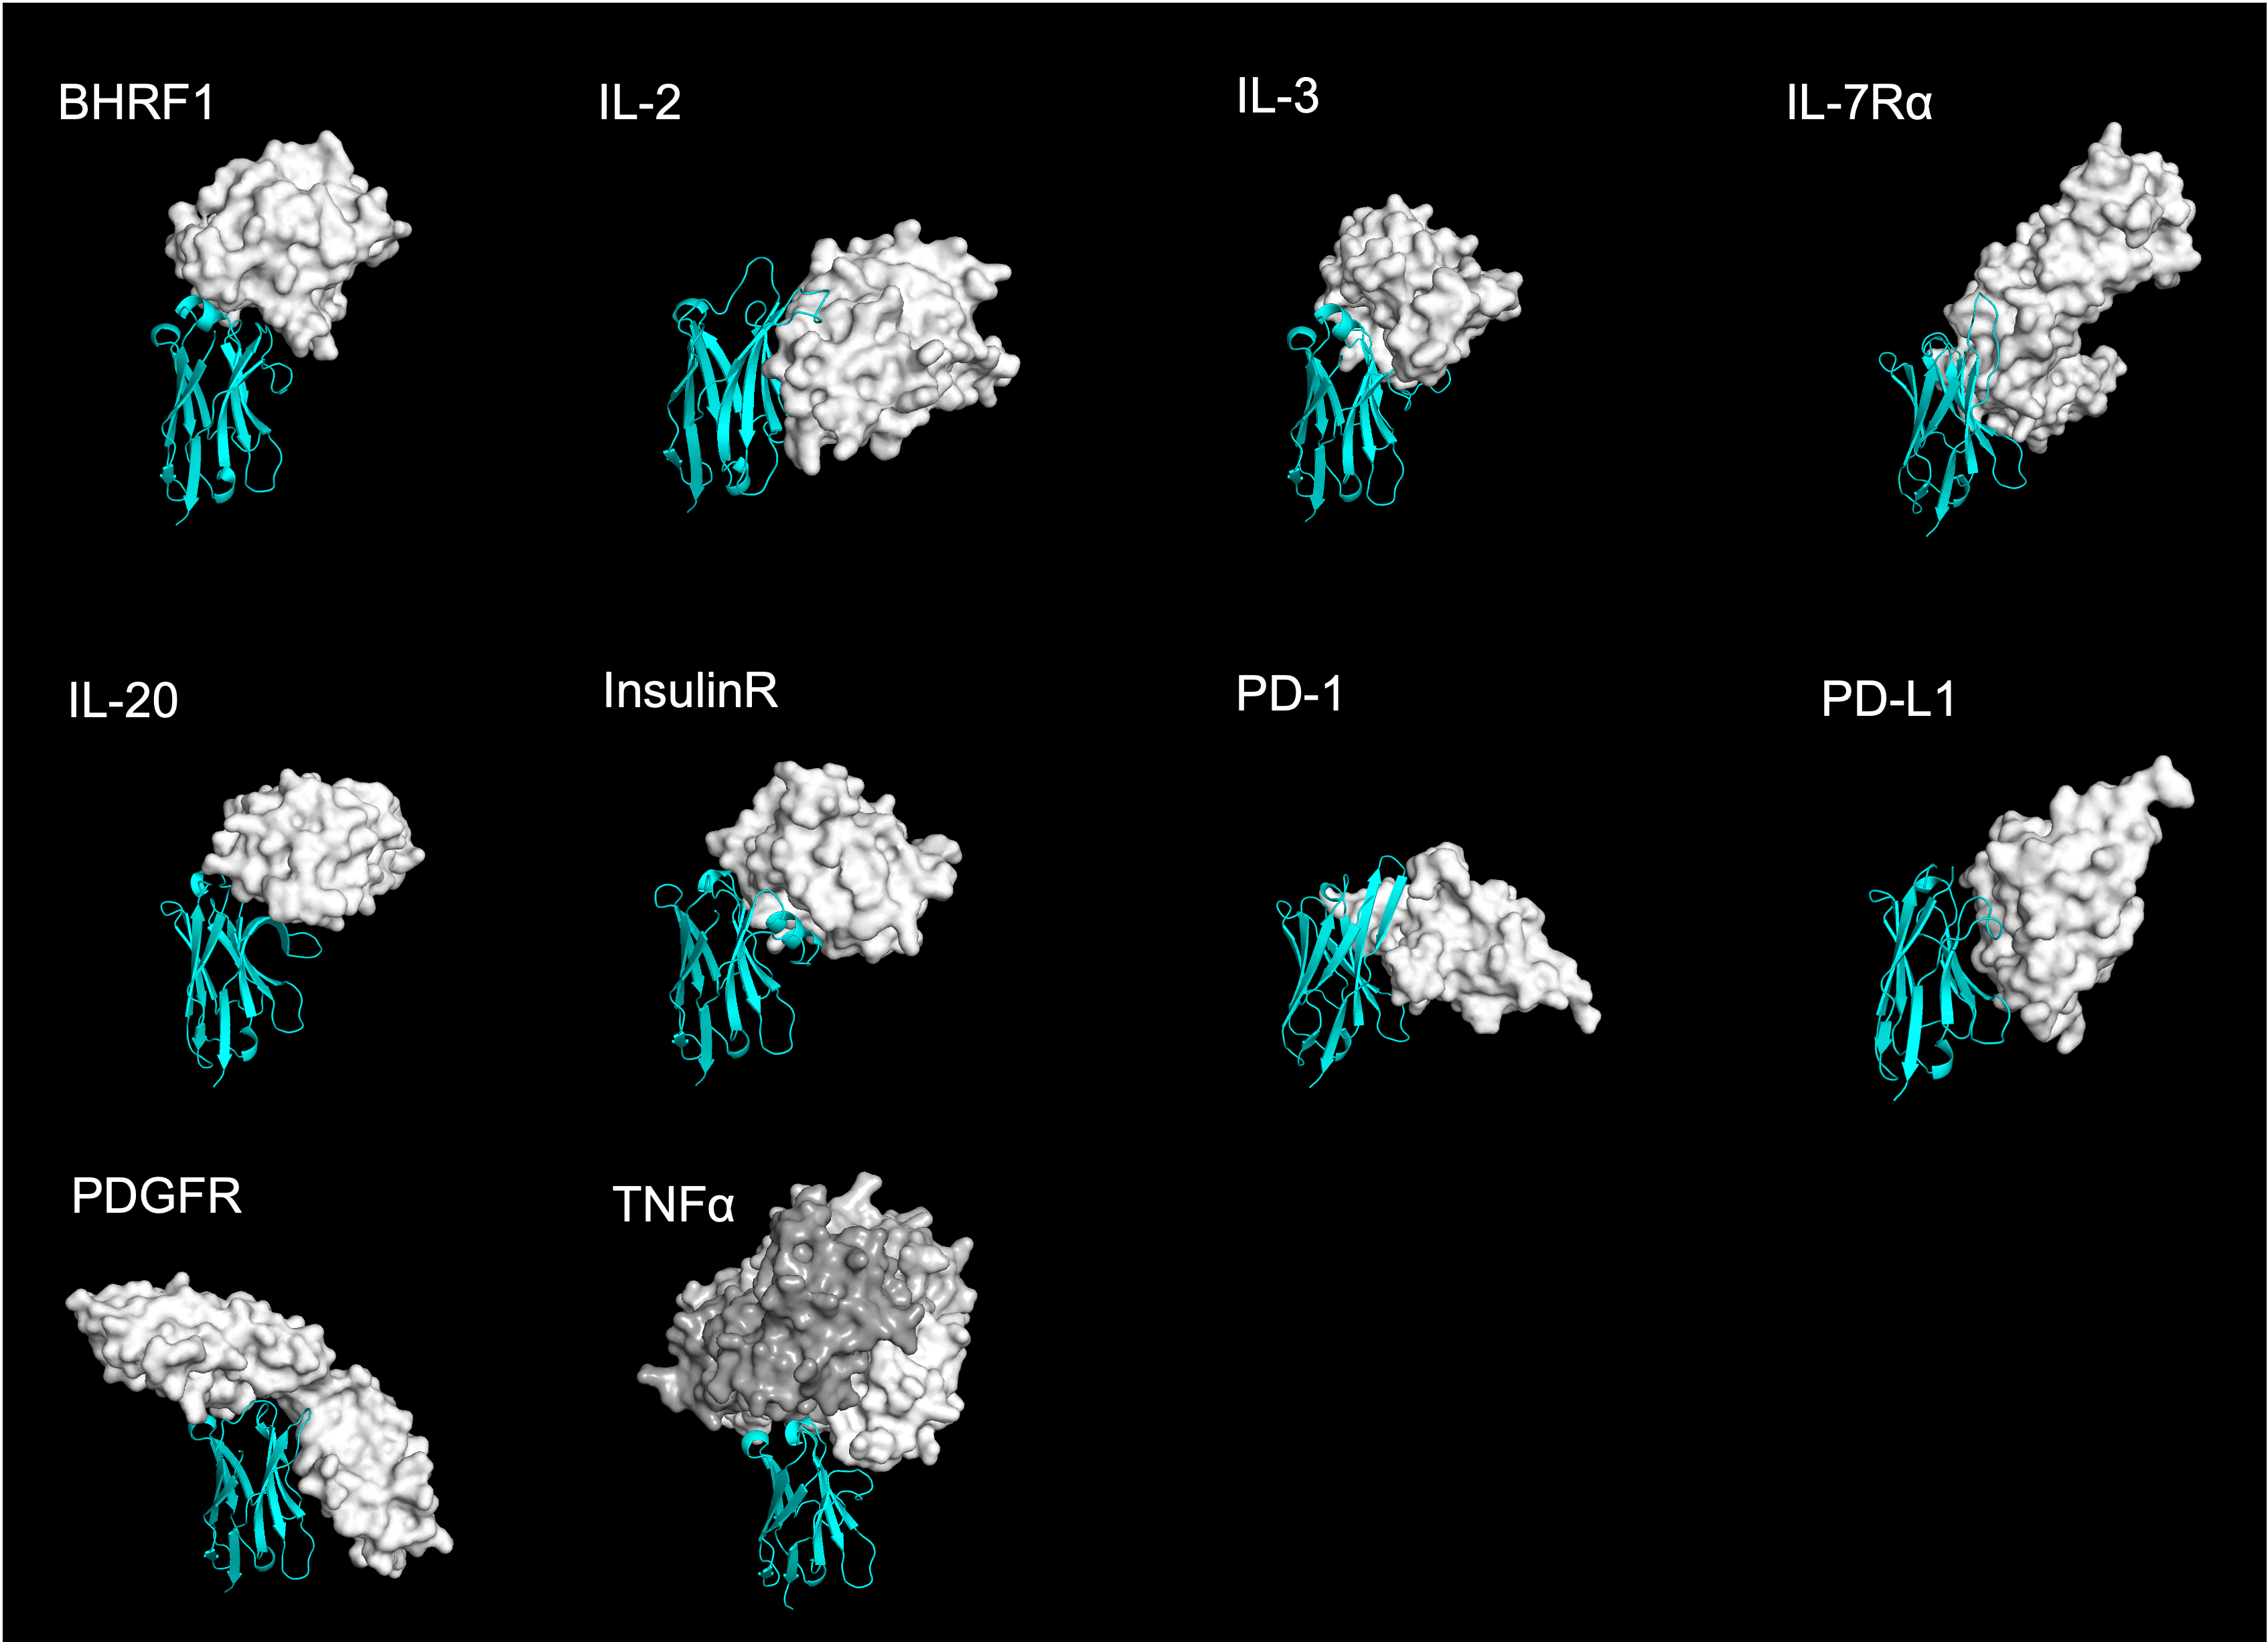
\includegraphics[width=\textwidth]{fig1.png}
  \caption{Predicted structures of the top-ranked VHH binder (cyan) in complex with each of the ten successful targets (white).}
\end{figure}

\section{Introduction}
Therapeutic antibody discovery remains dominated by large-scale stochastic screening, including
animal immunization and display-library selection, often requiring experimental interrogation of
millions to billions of variants. Although these approaches have produced numerous successful
therapeutics, they offer limited control over epitope specificity and therapeutic properties as well as
impose substantial experimental and temporal costs. A central challenge in computational biologics
engineering is therefore whether antibody discovery can transition from stochastic screening toward
programmable molecular generation and optimization.

Recent advances in generative modeling have transformed de novo protein binder design,
with systems such as RFdiffusion \cite{rfdiffusion}, BindCraft \cite{bindcraft}, and AlphaProteo \cite{alphaproteo} demonstrating that
high-affinity binders can be computationally generated directly from target structure. Extending
these advances to antibodies, however, has proven substantially more difficult because antibody--
antigen recognition is dominated by conformationally flexible CDR loops and highly heterogeneous
binding interfaces. Nevertheless, recent systems including Chai-2 \cite{chai2}, Germinal \cite{germinal}, BoltzGen \cite{boltzgen},
and GeoFlow-V3 \cite{geoflowv3} have begun to demonstrate proof-of-concept de novo antibody and nanobody
discovery.

Despite these advances, practical low-throughput antibody discovery remains unresolved.
Most current systems exhibit inconsistent success across targets, require substantial experimental
exploration, or have yet to demonstrate robust performance on difficult therapeutic antigens. In
particular, few studies have reported broad target-level success while experimentally testing only
tens of candidates per target.

Here we present MMDesign, a hallucination-guided de novo VHH discovery platform designed
to operate at experimentally tractable scales. Starting from only a target protein and specified epitope
residues, MMDesign combines sequence and structure co-generation with multi-tier computational
filtering to produce only tens of experimental candidates per target. We systematically evaluated
MMDesign across 11 therapeutically relevant targets spanning cytokines, immune checkpoints,
receptors, a viral protein, and a surface antigen. Experimental testing of only 14--50 candidates
per target yielded confirmed binders for 10 of 11 targets (90.9\%), with best measured affinities
ranging from picomolar to nanomolar levels. Notably, MMDesign achieved a 50\% hit rate on TNF$\alpha$,
a trimeric cytokine target that has proven difficult for prior low-throughput de novo VHH discovery
efforts [4, 6]. Together, these results suggest that generative nanobody discovery is beginning to
transition from proof-of-concept demonstrations toward a practical therapeutic discovery modality.

\section{Results}

\subsection{Practical De Novo VHH Discovery Across Therapeutically Diverse Targets}
To evaluate whether generative nanobody discovery can operate at experimentally practical scales,
we systematically evaluated MMDesign across 11 therapeutically relevant targets while experimentally testing only 14--50 candidates per campaign.

\textbf{Target diversity and structural complexity of the benchmark panel.} The target panel evaluated
in this study spans a broad range of therapeutically relevant protein classes and represents one of
the most structurally and biologically diverse benchmark sets reported for recent de novo antibody
or nanobody design systems. The eleven targets include cytokines (TNF$\alpha$, IL-2, IL-3, IL-20),
immune checkpoints (PD-1, PD-L1), receptor ectodomains (InsulinR, PDGFR, IL-7R$\alpha$), a viral protein
(BHRF1), and a surface antigen (CD7), collectively covering immunology, oncology, metabolism,
and infectious disease applications. Unlike many recent generative antibody-design studies that
focus primarily on a limited set of demonstration antigens, the MMDesign panel more closely
resembles the diversity encountered in real therapeutic biologics discovery.

Importantly, the benchmark diversity extends beyond biological categories and includes substantial variation in interface geometry and binding difficulty. TNF$\alpha$ represents a particularly
challenging case because it forms a homotrimeric cytokine complex with a shallow and solventexposed binding surface, a target class that has historically proven difficult for low-throughput
generative binder design. Receptor targets such as InsulinR, PDGFR, and IL-7R$\alpha$ introduce additional complexity through their large, flexible ectodomains and heterogeneous surface topologies.
Together, these targets span multiple binding regimes, including shallow exposed grooves, flexible
receptor interfaces, checkpoint interaction surfaces, and viral epitopes. As a result, the MMDesign
benchmark evaluates not only whether the platform can generate binders, but also whether it can
generalize across structurally distinct and therapeutically realistic antigen classes.

Candidate VHHs were generated through hallucination-guided sequence--structure optimization followed by multi-tier computational filtering incorporating structural reliability analysis,
sequence naturalness evaluation, and physics-based interface scoring.

Across the 11 campaigns, confirmed specific binders were obtained for 10 targets (90.9\%).
Experimental testing involved only tens of candidates per target, yet yielded per-target hit rates
ranging from 2.3\% to 86.7\% (Table~\ref{tab:validation}). Best measured affinities ranged from picomolar to micromolar
levels, with several campaigns producing binders in the low- to mid-nanomolar regime. In all
successful campaigns, predicted complex structures indicated direct contacts between designed
CDR residues and the user-specified epitope hotspot residues.

Among all targets, PD-L1 achieved the highest hit rate, with 26 of 30 tested candidates confirmed
as specific binders and a best measured $K_D$ of 7.2~nM. Additional campaigns yielded multiple
confirmed binders across diverse antigen classes, including InsulinR (5/25, best $K_D$ 25~nM), BHRF1
(5/35, best $K_D$ 282~nM), IL-2 (5/50, best $K_D$ 138~nM), and IL-3 (2/25, best $K_D$ $\sim$200~nM). Single
confirmed binders were also identified for PDGFR, IL-7R$\alpha$, IL-20, and PD-1. Only one target, CD7,
yielded no confirmed binders under the current pipeline configuration.

\begin{table}[!htbp]
\centering
\begin{tabular}{llcccc}
\toprule
Target & Category & Hits / Tested & Hit Rate (\%) & Best $K_D$\\
\midrule
PD-L1    & Checkpoint      & 26 / 30 & 86.7 & 7.2 nM\\
TNF$\alpha$  & Cytokine        & 7 / 14  & 50.0 & 51 pM$^{\ast}$\\
InsulinR & Receptor        & 5 / 25  & 20.0 & 25 nM\\
BHRF1    & Viral protein   & 5 / 35  & 14.3 & 282 nM\\
IL-2     & Cytokine        & 5 / 50  & 10.0 & 138 nM\\
IL-3     & Cytokine        & 2 / 25  & 8.0  & $\sim$200 nM\\
PDGFR    & Receptor        & 1 / 25  & 4.0  & 150 nM\\
IL-7R$\alpha$ & Receptor    & 1 / 25  & 4.0  & 408 nM\\
IL-20    & Cytokine        & 1 / 40  & 2.5  & 6.5 $\mu$M\\
PD-1     & Checkpoint      & 1 / 44  & 2.3  & 38 nM\\
\midrule
CD7      & Surface antigen & 0 / 25  & 0    & ---\\
\bottomrule
\end{tabular}
\caption{Experimental validation results across all 11 target campaigns. Hit Rate = confirmed
hits / candidates tested. Best $K_D$ measured by BLI unless otherwise noted.}
\footnotesize{$^{\ast}$ Apparent $K_D$ reflects avidity due to the trimeric nature of TNF$\alpha$ analyte.}
\label{tab:validation}
\end{table}

Together, these results demonstrate that MMDesign can achieve broad target-level success while
experimentally testing only tens of candidates per target, suggesting that generative VHH discovery
may increasingly operate at experimentally tractable scales.

Structural analysis of the designed complexes indicates these binders are genuinely novel: 9
of the 11 targets have no known VHH complex in the PDB, and the designs occupy previously
uncharacterized binding-pose space (Appendix~\ref{app:C}). At the same time, for targets where validated
references exist, the designs converge on the same functional epitopes despite entirely de novo
CDRs---including recovery of the natural PD-1:PD-L1 inhibitory interface.

\subsection{MMDesign Achieves a 50\% Hit Rate on the Difficult TNF$\alpha$ Target}
TNF$\alpha$ is a homotrimeric cytokine whose shallow and solvent-exposed binding surface has historically proven difficult for low-throughput de novo VHH discovery approaches [4, 6]. Prior generative
nanobody campaigns reported in the literature have failed to produce confirmed binders against
this target under similarly limited experimental throughput settings.

To evaluate MMDesign on this challenging system, all three CDR loops were optimized through
the hallucination-guided generation pipeline, and 14 candidates were selected for experimental
characterization. Seven designs (50\%) exhibited clear and specific target binding by BLI. The lead
molecule achieved an apparent $K_D$ of 51 pM, noting that this value reflects avidity enhancement
associated with the trimeric TNF$\alpha$ analyte.

The TNF$\alpha$ campaign is particularly notable because it demonstrates substantial enrichment
under extremely limited experimental exploration. Rather than requiring large-scale stochastic
screening, the computational pipeline successfully narrowed tens of thousands of generated candidates to a small experimentally tractable set enriched for true binders. These results suggest that
AI-guided generative discovery may increasingly access difficult therapeutic geometries that have
historically resisted low-throughput discovery workflows.

Representative predicted structures and BLI sensorgrams for selected targets are shown in
Figure~\ref{fig:validation}.

\subsection{Designed VHHs Exhibit Favorable Preliminary Developability Characteristics}
In addition to binding activity, many designed VHHs exhibited encouraging preliminary developabilityrelated properties. Expression yields across campaigns demonstrated that numerous candidates
could be robustly expressed as VHH-Fc constructs in CHO cells (Figure~\ref{fig:expression}). Size-exclusion chromatography further showed that many purified candidates remained predominantly monomeric
with limited aggregation signatures (Figure~\ref{fig:sec}).

To assess preliminary specificity characteristics, a subset of designed VHHs was evaluated for
off-target binding against human serum albumin (HSA), the most abundant protein in plasma and
a common source of non-specific interactions in therapeutic antibody development. Across all
tested candidates, BLI responses against HSA remained minimal at micromolar concentrations,
with no measurable evidence of strong non-specific binding (Figure~\ref{fig:hsa}). Additional poly-reactivity
ELISA experiments against insulin and dsDNA similarly indicated low levels of broad non-specific
reactivity.

Although these experiments do not constitute a comprehensive therapeutic developability
assessment, they suggest that MMDesign can generate experimentally tractable antibody-like
molecules rather than merely isolated binding sequences. These observations suggest that future generative biologics systems may increasingly optimize simultaneously for binding activity,
specificity, expression, stability, and downstream therapeutic developability characteristics.

\begin{figure}[!htbp]
  \centering
  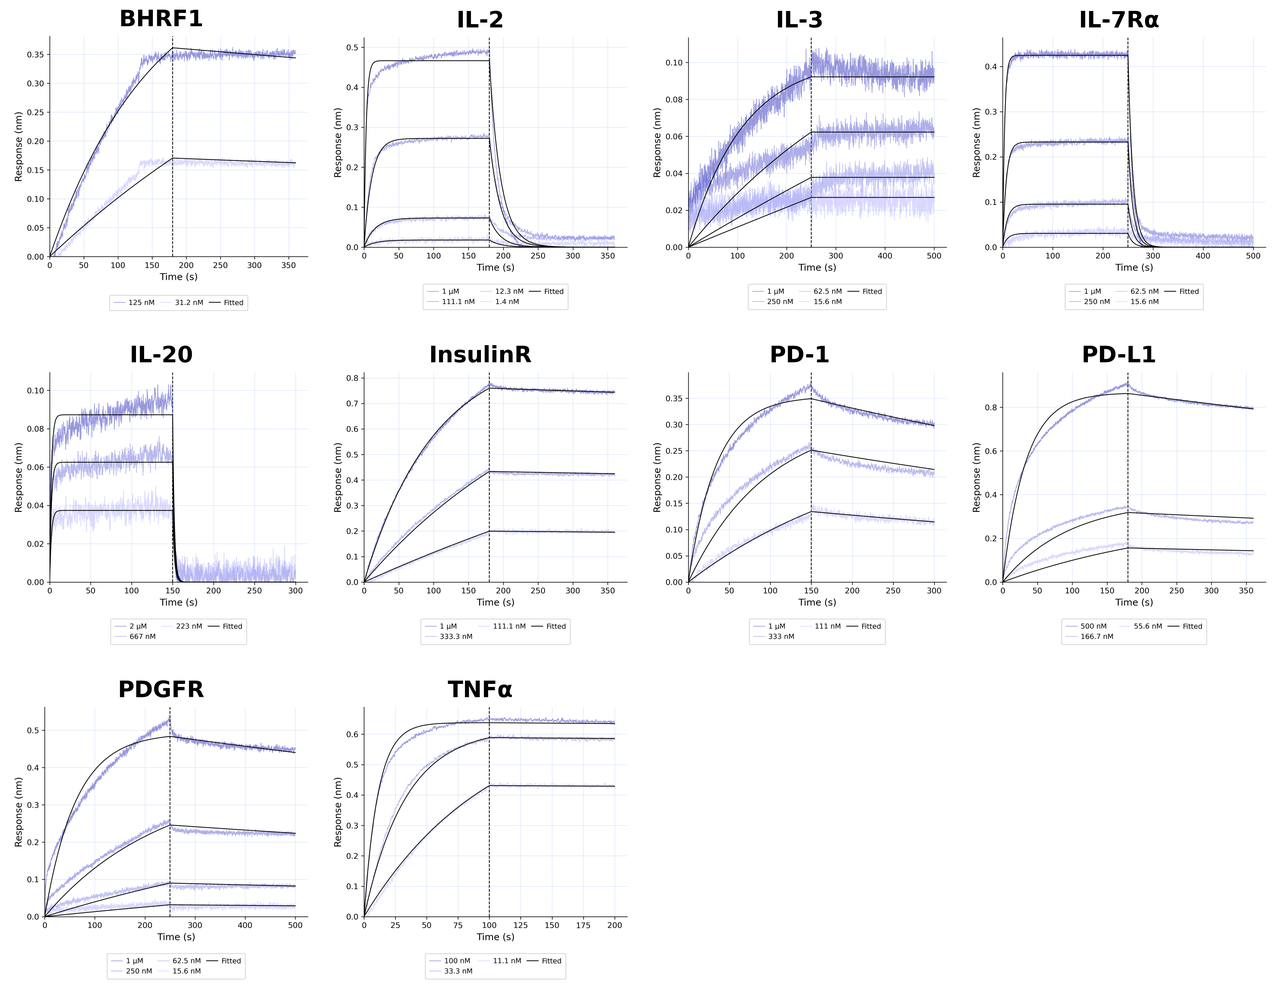
\includegraphics[width=\textwidth]{fig2.png}
  \caption{Experimental validation of computationally prioritized VHH candidates. For each target,
the predicted VHH--antigen complex structure (left) and multi-concentration BLI sensorgrams with
1:1 global fit (right) are shown.}
  \label{fig:validation}
\end{figure}

\subsection{Multi-Tier Computational filtering Enriches Experimental Hit Discovery}
A post-hoc analysis of the computational filtering pipeline revealed that no single metric alone was
sufficient to robustly identify the highest-quality binders across targets. In particular, structureprediction confidence metrics such as ipTM and pLDDT showed limited correlation with experimentally measured affinity among confirmed binders, consistent with previous observations that
confidence metrics may function primarily as coarse binary indicators of binding compatibility
rather than quantitative affinity predictors.

Instead, the layered integration of multiple filtering criteria consistently produced stronger
enrichment than any individual metric in isolation. The filtering cascade incorporated four major
components: (i) structural confidence evaluation, (ii) reproducibility analysis across random seeds
and prediction models, (iii) protein language model--based sequence naturalness assessment, and
(iv) in-house statistical physics--aware interface scoring. Designs passing all filtering stages were
substantially enriched for experimentally confirmed binders relative to candidates selected using
any single criterion alone.

These observations suggest that the central challenge in practical AI-native biologics discovery
is not merely generating candidate sequences, but enriching true binders sufficiently to minimize
experimental burden. In this context, multi-objective computational prioritization appears to play a
critical role in enabling experimentally practical low-throughput discovery workflows.

\begin{figure}[!htbp]
  \centering
  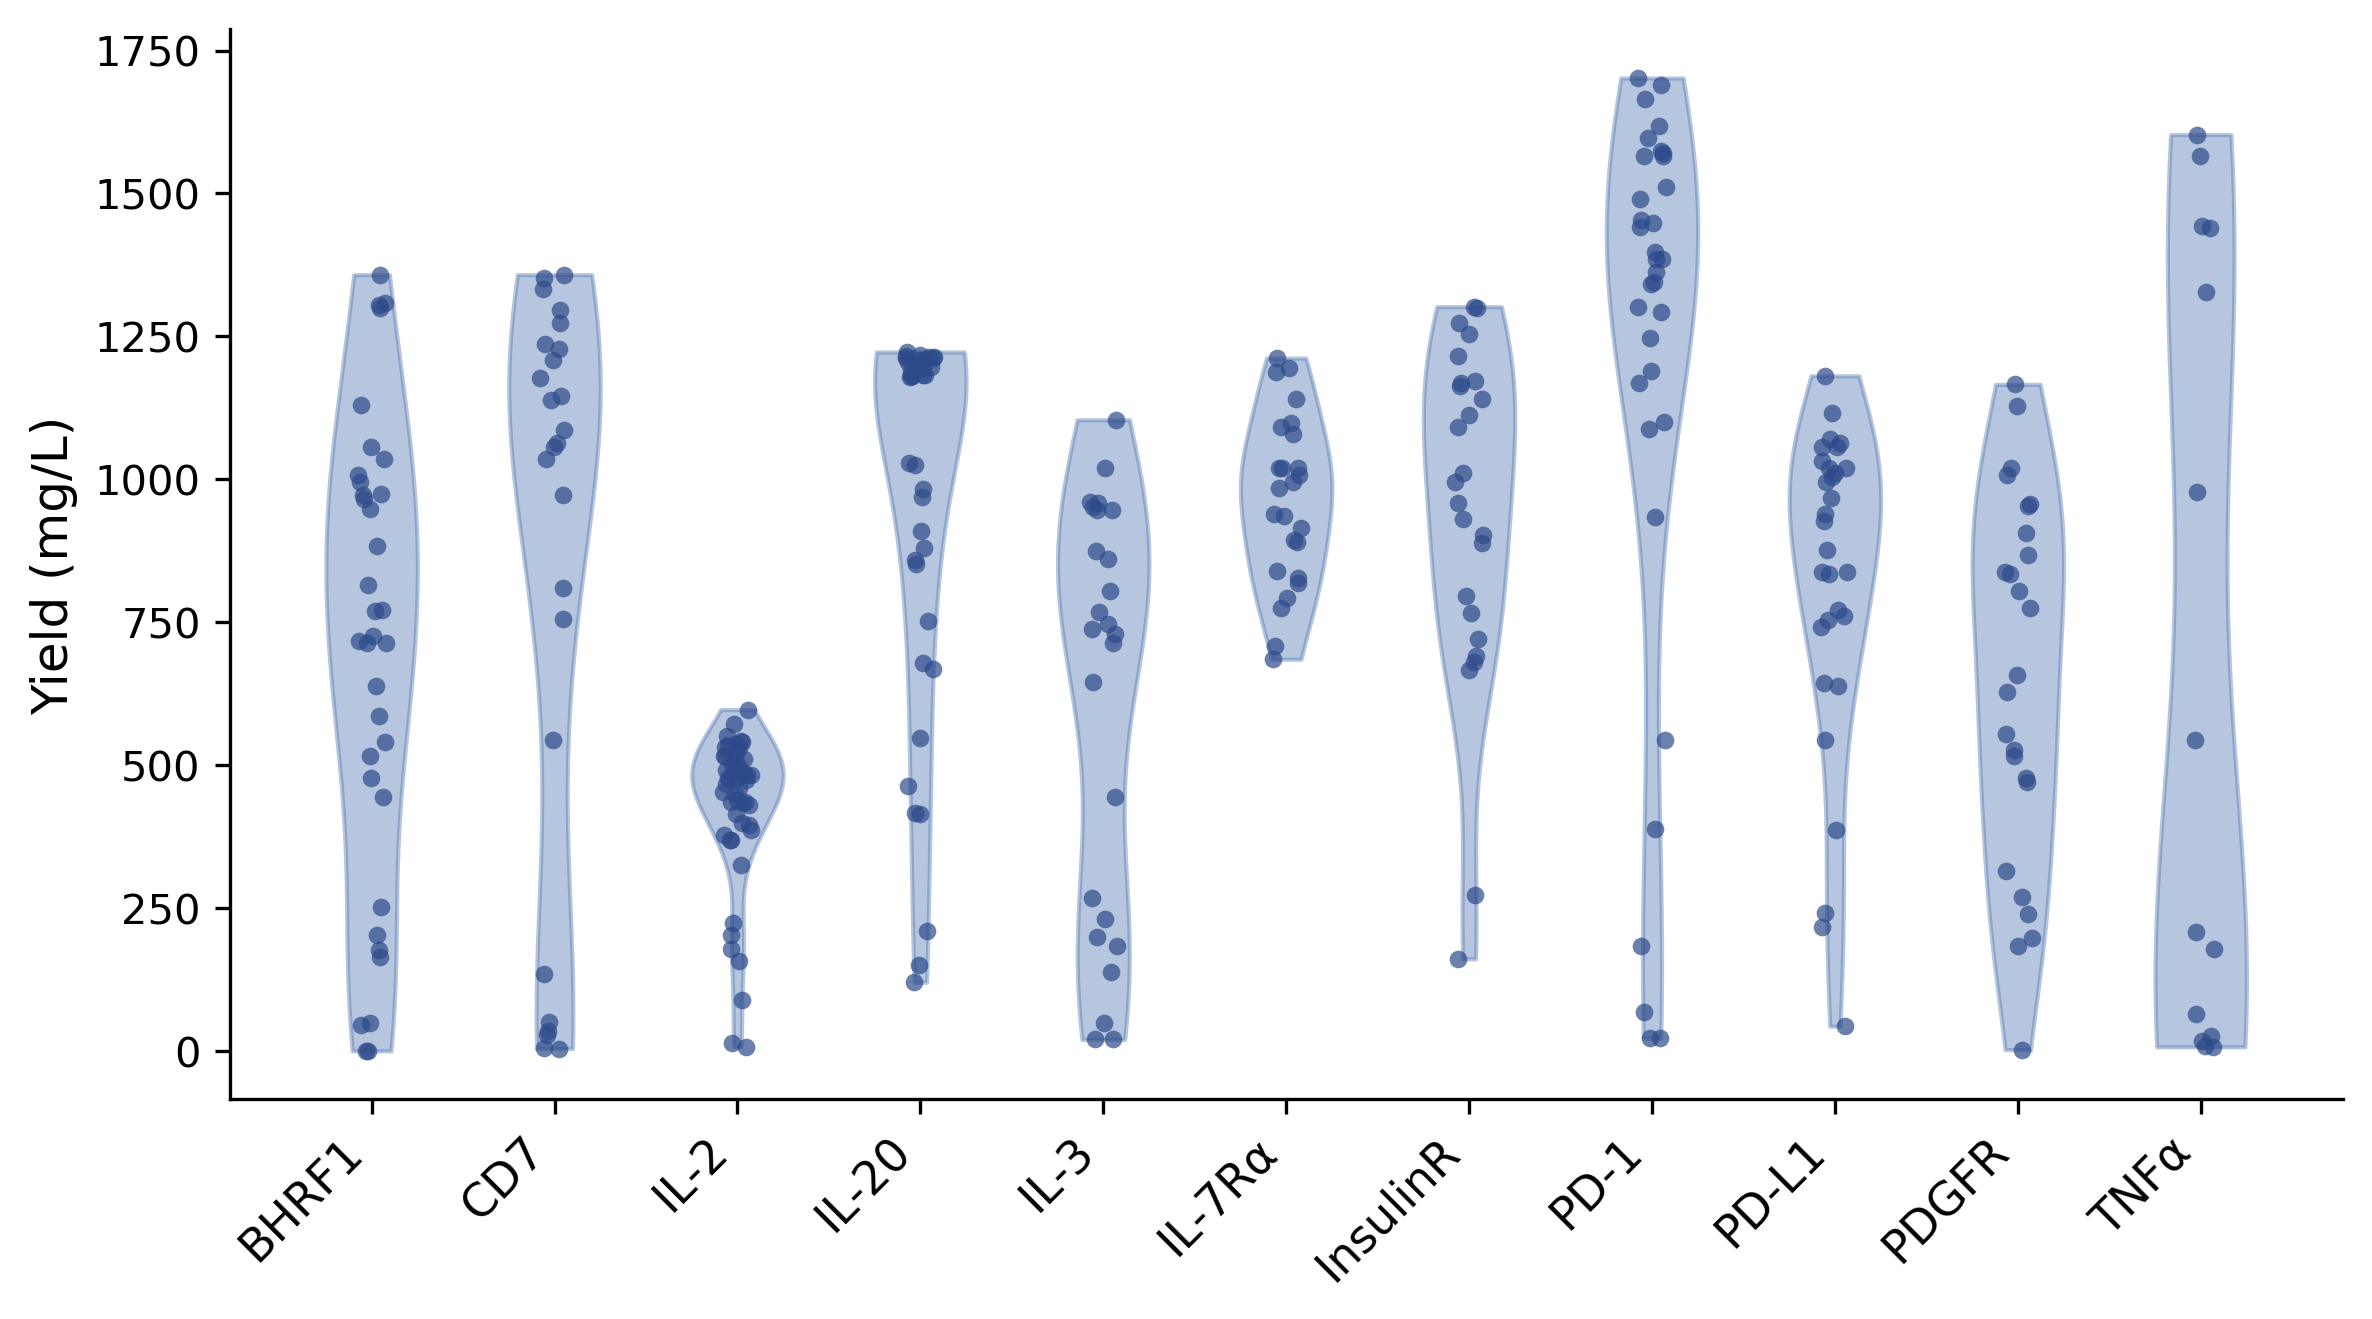
\includegraphics[width=\textwidth]{fig3.png}
  \caption{Expression yields (mg/L) of VHH-Fc constructs across all target campaigns. Each data
point represents one designed candidate expressed in CHO at 10~mL scale.}
  \label{fig:expression}
\end{figure}

\begin{figure}[!htbp]
  \centering
  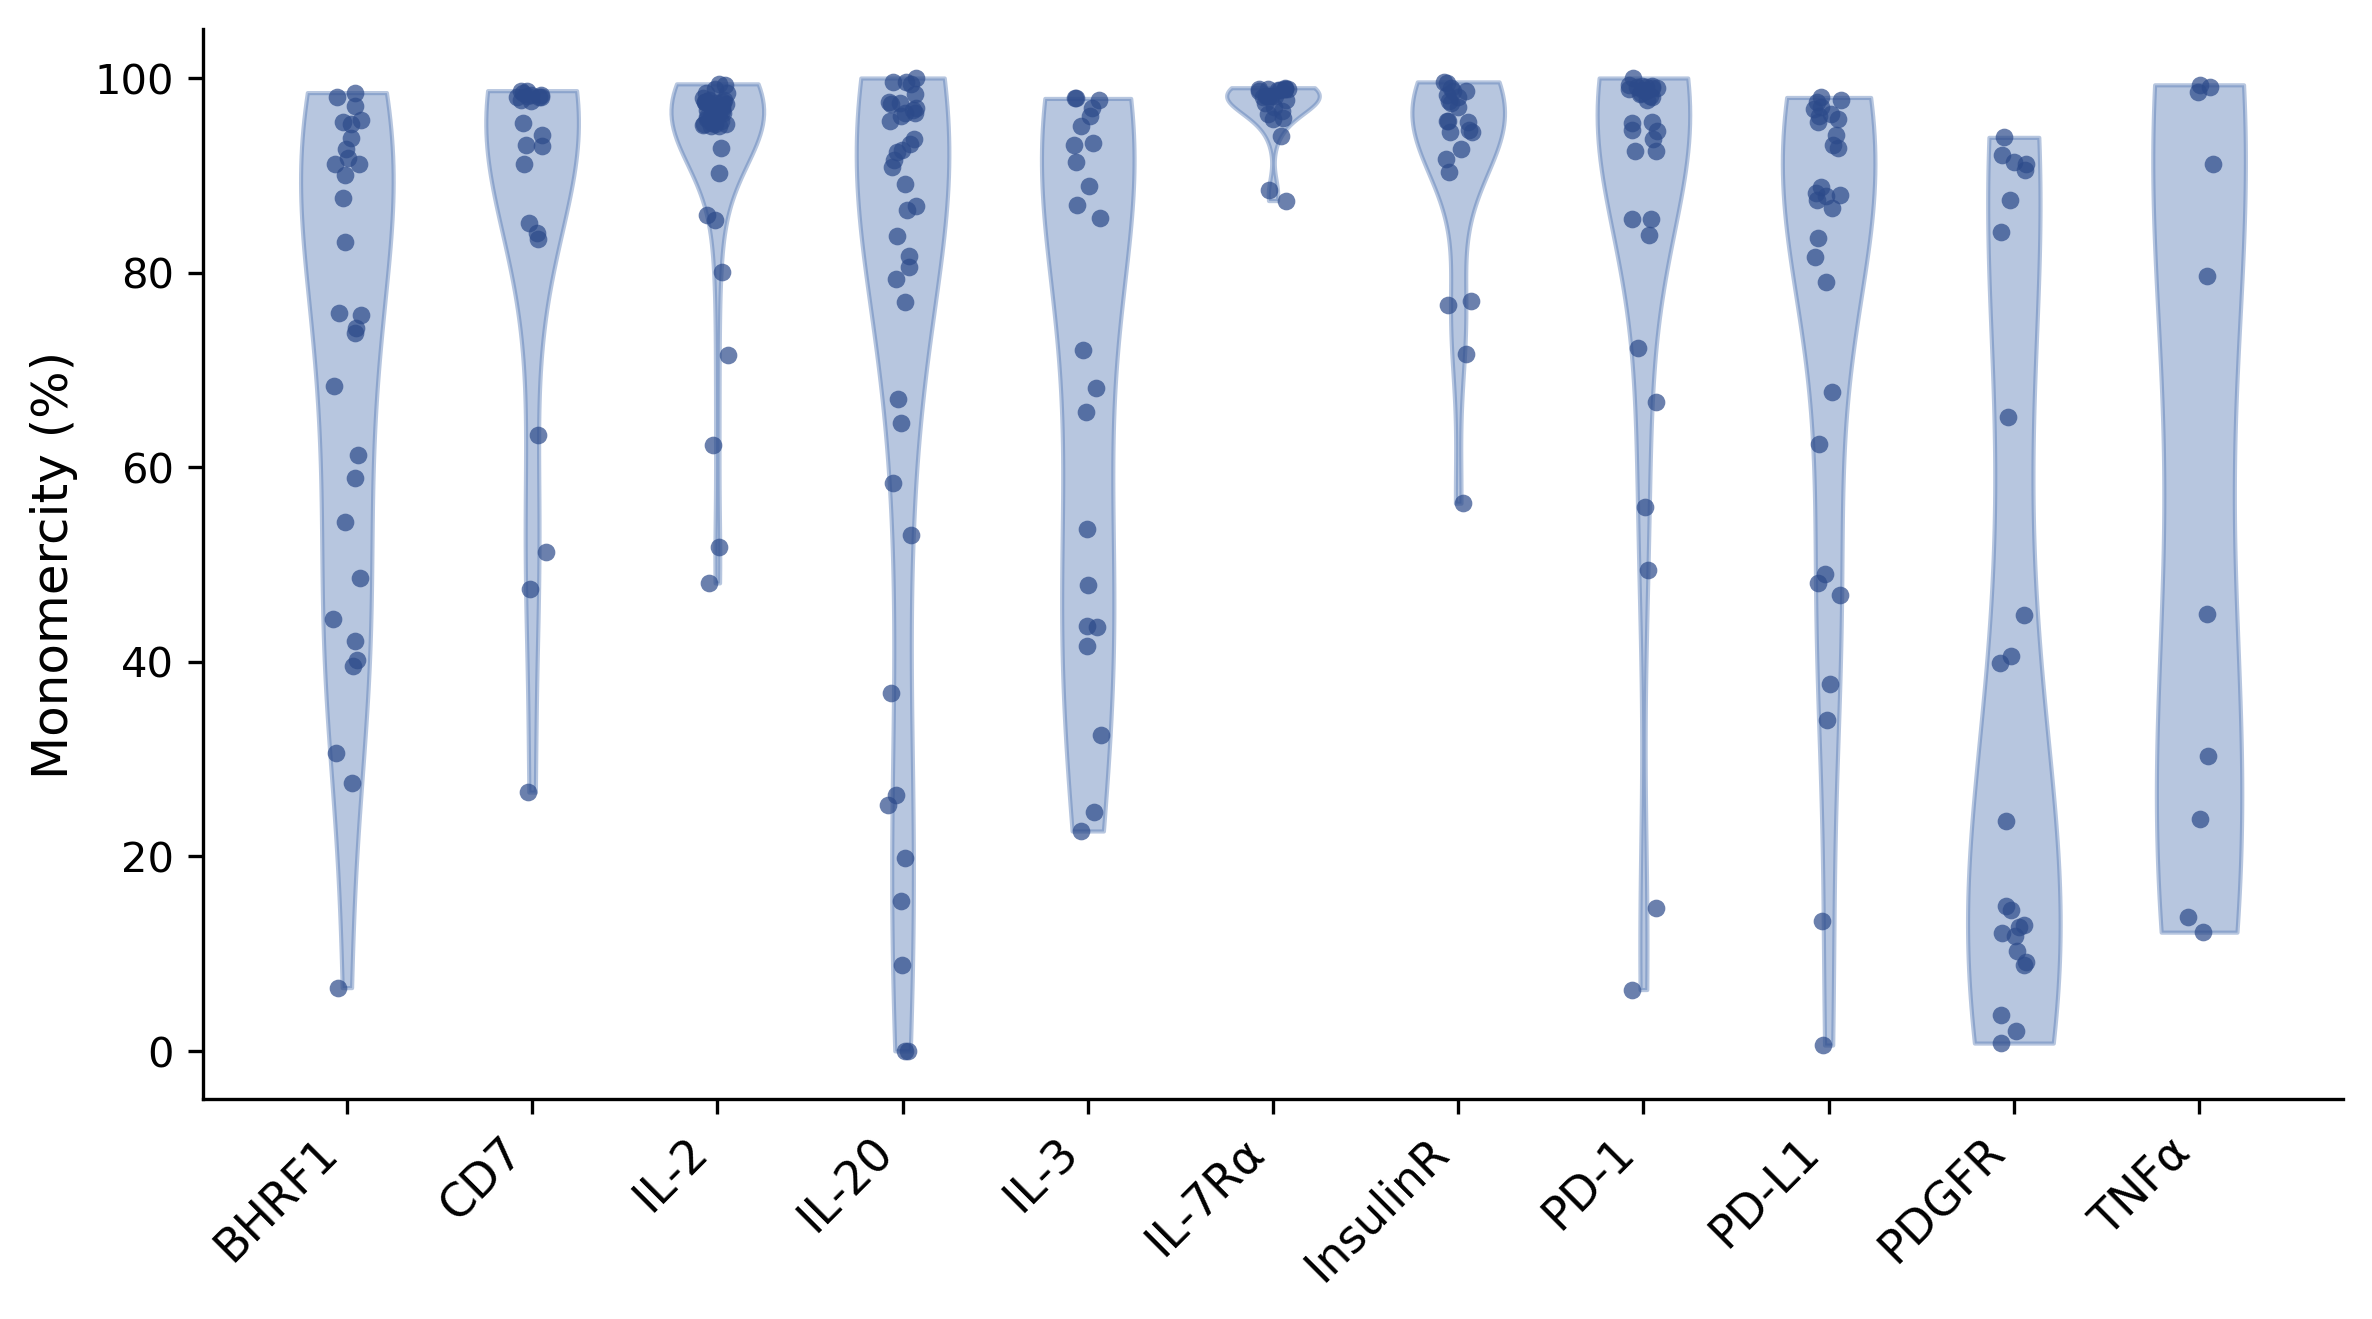
\includegraphics[width=0.8\textwidth]{fig4.png}
  \caption{SEC-HPLC chromatograms of representative VHH-Fc candidates. The dominant peak
indicates the monomeric VHH-Fc species; minor peaks, if present, correspond to aggregates or
degradation products.}
  \label{fig:sec}
\end{figure}

\begin{figure}[!htbp]
  \centering
  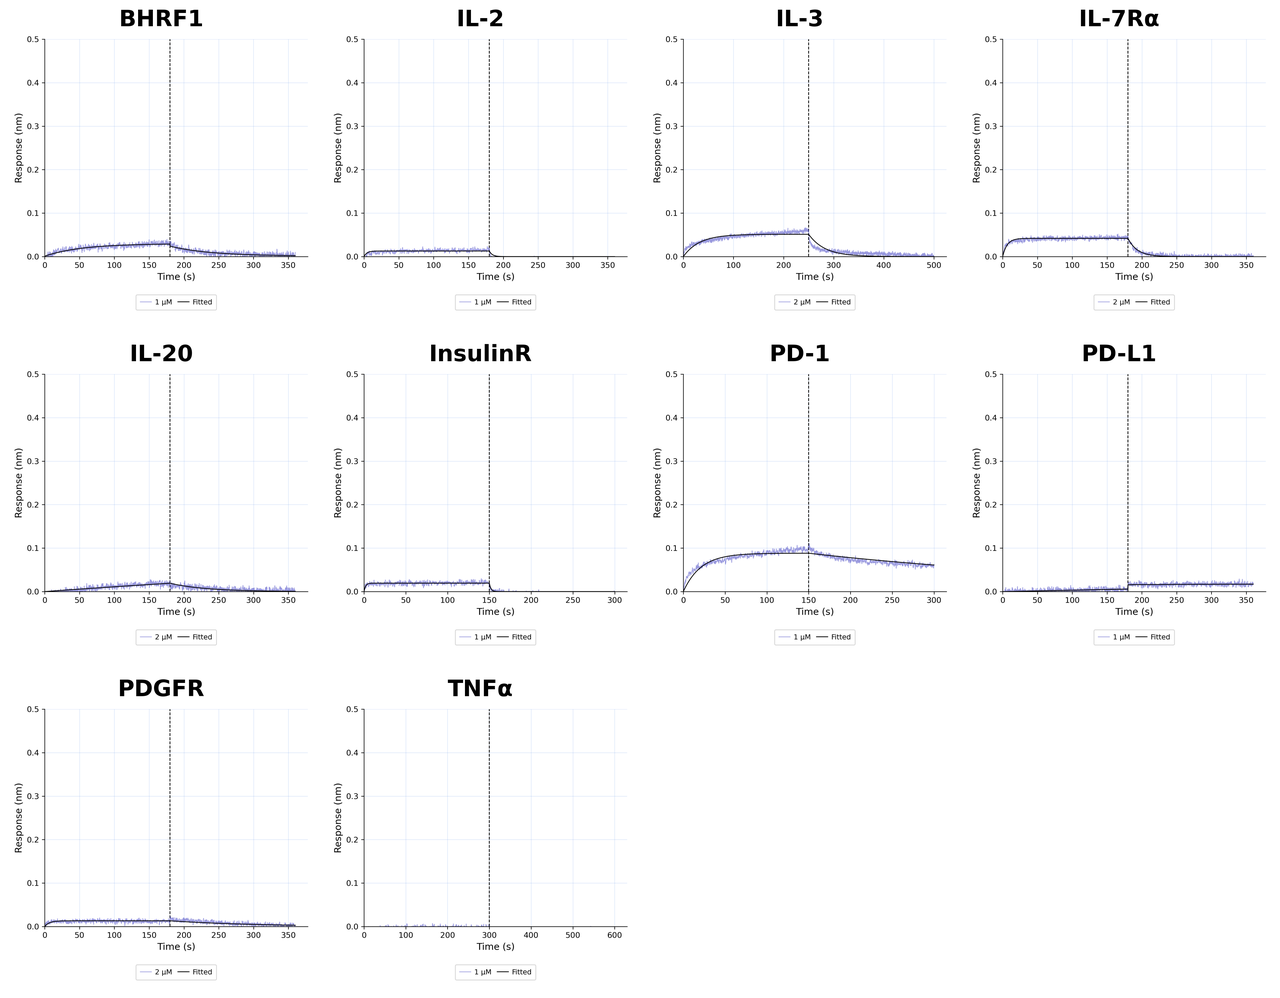
\includegraphics[width=\textwidth]{fig5.png}
  \caption{BLI sensorgrams of seven designed VHH candidates against HSA at 1--2~$\mu$M. The dashed
vertical line marks the transition from association to dissociation. Blue: experimental response;
black: 1:1 kinetic fit.}
  \label{fig:hsa}
\end{figure}

\subsection{MMFold Achieves High Accuracy on Antibody--Antigen Complex Prediction}
Because hallucination-guided optimization depends on the quality of the underlying structureprediction confidence landscape, we evaluated MMFold on the FoldBench \cite{foldbench} antibody--antigen
benchmark dataset. MMFold is a proprietary all-atom structure prediction model inspired by the
AlphaFold 3 architecture \cite{alphafold3} and trained with enhanced antibody--antigen modeling capability.
MMFold was trained on Protein Data Bank \cite{pdb} entries released before September 30, 2021.

Across 172 antibody--antigen interfaces, MMFold achieved an overall DockQ \cite{dockq} acceptableor-better success rate of 68.6\% for Top-1 predictions, compared with 47.9\% for AlphaFold 3 on the
same benchmark. Improvements were also observed across medium- and high-quality DockQ
thresholds. When expanded to Top-5 predictions, MMFold further increased acceptable-or-better
performance to 75.6\% (Figure~\ref{fig:dockq}). The accuracy of MMFold also scales well along with the number
of sampled predictions. For example, when a few hundred seeds are used, MMFold may achieve
high resolution success rate of around 50\% for Top-5 predictions.

Several recently released structure-prediction models were not included in this comparison.
Boltz-2 \cite{boltz2} was excluded because its more recent training cutoff overlaps with part of the FoldBench
release window, which precludes a leakage-free evaluation on this benchmark; notably, the authors
themselves report that ``Boltz-2 shows an improvement over Boltz-1 while still lagging behind
AlphaFold3.'' Protenix-v2 \cite{protenixv2} reports a DockQ acceptable-or-better success rate of 65\% for Top-1
predictions, but this figure was obtained on a 103-PDB-ID (160-interface) subset of the FoldBench
antibody--antigen benchmark rather than the full 113-PDB-ID (172-interface) set used here. It is
therefore not directly comparable to the results in Figure~\ref{fig:dockq} and is not included.

\begin{figure}[!htbp]
  \centering
  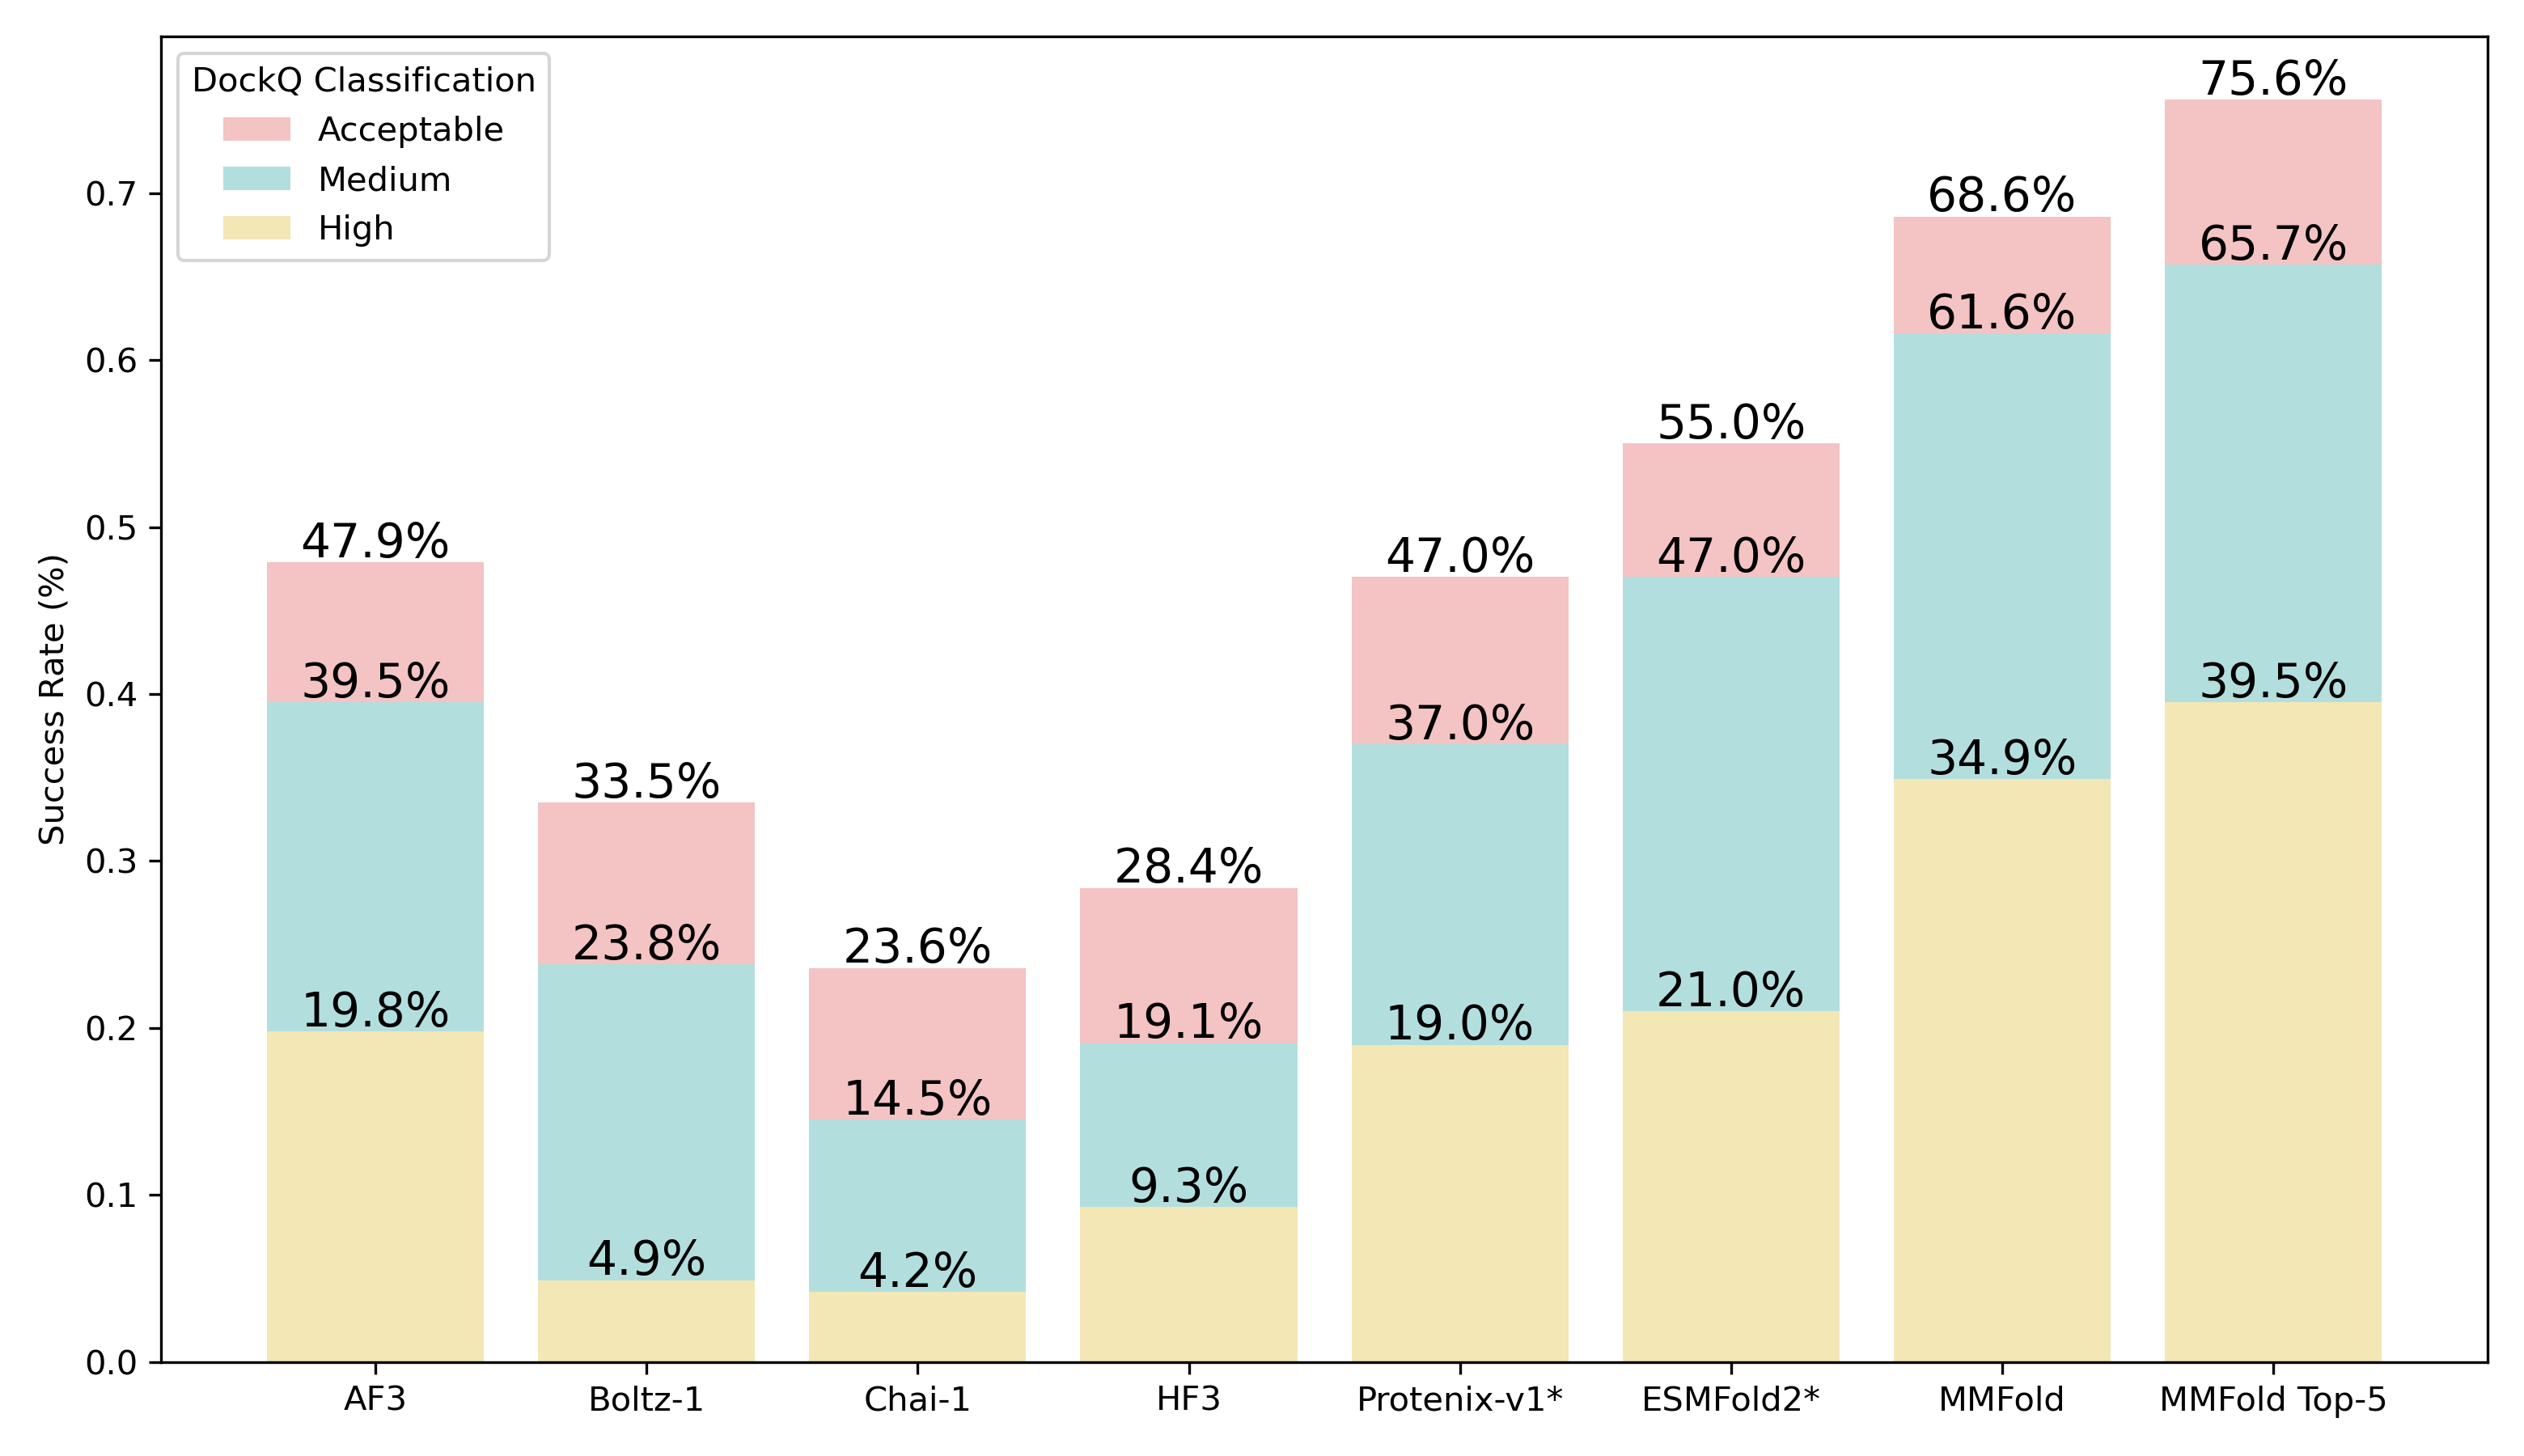
\includegraphics[width=0.9\textwidth]{fig6.png}
  \caption{Performance comparison of MMFold against leading structural prediction models based
on DockQ classification. The stacked bar chart illustrates the cumulative success rates (\%) at
High (yellow), Medium (teal), and Acceptable (pink) quality thresholds. MMFold demonstrates
significantly higher Top-1 and Top-5 success rates across all quality tiers compared to baselines
including AlphaFold 3, Boltz-1, Chai-1, HelixFold3, Protenix-v1 \cite{protenixv1}, and ESMFold2 \cite{esmfold2}. Values
marked with an asterisk (Protenix-v1* and ESMFold2*) are reported and infered from the ESMFold2
paper \cite{esmfold2} on the FoldBench antibody--antigen benchmark; the ESMFold2 result corresponds to its
20-loop inference setting. All other models were evaluated here under a single, consistent protocol.}
  \label{fig:dockq}
\end{figure}

Representative case studies demonstrated substantially improved interface modeling relative
to AlphaFold 3 for multiple antibody--antigen complexes, including examples in which MMFold
accurately recovered binding geometries that were poorly modeled by baseline systems (Figure~\ref{fig:cases}).
Detailed benchmark procedures and additional benchmarking analyses are provided in the Supplementary Information.

Although the current study does not directly establish a causal relationship between structureprediction accuracy and experimental discovery success, these results suggest that improved
antibody-antigen structure modeling may provide higher-quality confidence landscapes for downstream generative biologics optimization workflows.

\begin{figure}[!htbp]
  \centering
  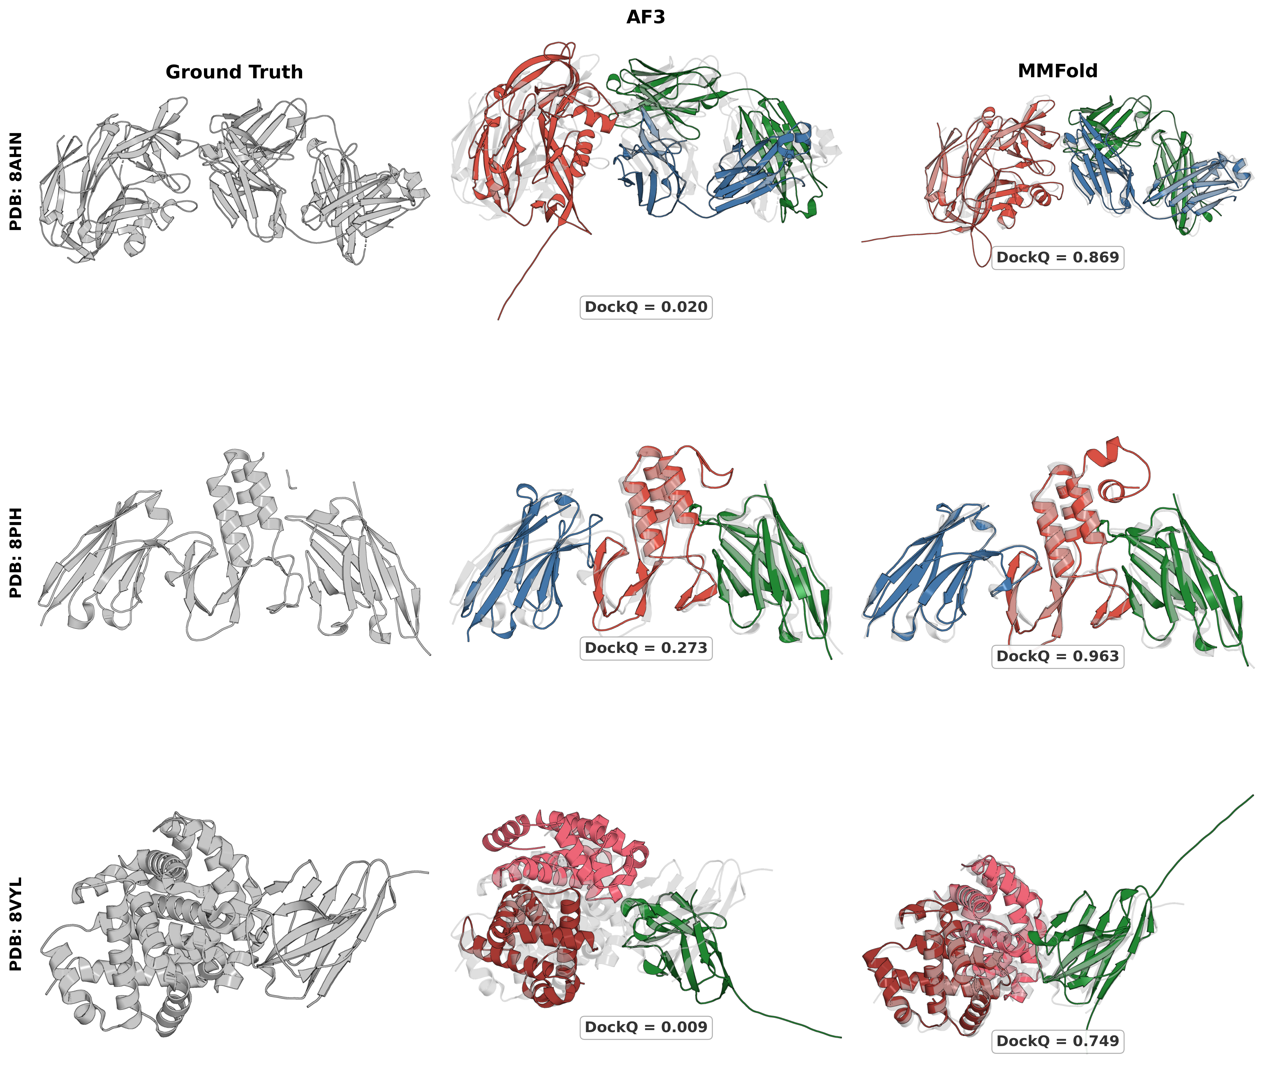
\includegraphics[width=0.7\textwidth]{fig7.png}
  \caption{Case studies illustrating the prediction accuracy of antibody--antigen protein complexes.
The experimental ground truth (left column) is depicted in solid gray. In the prediction panels
(middle: AlphaFold 3; right: MMFold), predicted models are color-coded by subunit---with antigens
in red---and superimposed onto the translucent ground truth to visualize structural deviations.}
  \label{fig:cases}
\end{figure}

\section{Discussion}
Recent advances in generative modeling have established the possibility of de novo antibody and
nanobody generation. The results presented here suggest that the field may now be beginning
to transition from proof-of-concept demonstrations toward experimentally practical discovery
workflows. Across 11 therapeutically relevant targets, MMDesign produced confirmed binders for
10 targets while experimentally testing only 14--50 candidates per campaign, spanning cytokines,
immune checkpoints, receptors, a viral protein, and a surface antigen. These findings suggest that
generative VHH discovery can increasingly operate at experimentally tractable scales rather than
relying on massive stochastic screening campaigns.

A defining feature of practical AI-native biologics discovery may ultimately be the ability to
dramatically compress experimental screening burden while maintaining broad target-level success.
Conventional antibody discovery workflows, including animal immunization and display-library
screening, typically require exploration of millions to billions of variants and provide limited
control over epitope specificity. In contrast, MMDesign starts from only a target protein and userspecified epitope residues, computationally generates tens of thousands of candidate VHHs, and
narrows this space to only tens of experimental designs through layered computational enrichment.
More broadly, these results suggest a possible transition in biologics discovery from stochastic
experimental screening toward programmable molecular engineering.

\textbf{Sequence novelty of designed binders.} A key consideration for any generative design platform
is whether the output sequences represent genuinely novel molecules or merely recapitulate known
antibodies. The MMDesign generative core is a general-purpose all-atom structure-prediction
model that was not specifically fine-tuned on antibody--antigen complexes; the hallucination-based
optimization explores the model's confidence landscape without reference to any antibody sequence
database. Consequently, the generation process cannot, by construction, copy or derive sequences
from existing binders---whether deposited in public databases or disclosed in patent filings. CDR
similarity analysis (Appendix~\ref{app:A}) and structural comparison against SAbDab (Appendix~\ref{app:B}) confirm
that the designed sequences are substantially divergent from known antibodies, with framework regions preserving canonical VHH scaffold geometry (per-region C$\alpha$-RMSD consistently below 0.7~\AA{})
while CDR loops---particularly CDR3---adopt conformations largely absent from the experimental
database. Binding-pose comparison against known PDB complexes (Appendix~\ref{app:C}) provides further
evidence of structural novelty: 9 of the 11 targets have no nanobody complex in the PDB, so the
designed VHHs occupy previously uncharacterized structural space. Where validated references
do exist, the designs independently converge on the same functional epitopes despite entirely de
novo CDRs---the TNF$\alpha$ design recovers the 5M2J epitope (centroid distance 1.03~\AA{}), and the PD-1
design lands on the natural PD-1:PD-L1 interface (centroid distance 0.79~\AA{}, 14 of 24 contacts shared),
consistent with a competitive-inhibition mechanism.

The TNF$\alpha$ campaign is particularly notable in this context. TNF$\alpha$ is a homotrimeric cytokine with
a relatively shallow and solvent-exposed binding surface that has historically proven challenging for
low-throughput de novo VHH discovery efforts. In this study, experimental testing of only 14 candidates yielded 7 confirmed binders, corresponding to a 50\% hit rate, with the lead molecule reaching
an apparent $K_D$ of 51 pM in the avidity-enhanced trimeric setting. Although further characterization
will be required to evaluate the generality of this result, it suggests that hallucination-guided generation may begin to access difficult antigen geometries that have historically resisted computational
low-throughput discovery approaches.

An additional notable aspect of the current study is that many designed VHHs exhibited favorable preliminary developability-related properties beyond target binding alone. Across campaigns,
numerous candidates achieved robust recombinant expression in CHO cells, remained predominantly monomeric by SEC-HPLC, and showed minimal detectable cross-reactivity against HSA in
BLI assays. Although these measurements do not constitute a comprehensive developability assessment, they suggest that generative discovery systems may increasingly be capable of producing
experimentally tractable antibody-like molecules rather than merely isolated binding sequences.
More broadly, these observations raise the possibility that future generative antibody platforms
may optimize not only for binding activity, but simultaneously for expression, stability, specificity,
and downstream therapeutic developability.

The current study also highlights the potential importance of integrating generation and computational filtering within a unified workflow. Post-hoc analysis indicated that no individual metric
alone---including structure-prediction confidence measures such as ipTM or pLDDT---was sufficient
to robustly identify the highest-quality binders across targets. Instead, the layered combination of
structural reproducibility analysis, sequence naturalness evaluation, epitope-contact verification,
and physics-based interface assessment consistently provided stronger enrichment than any single
criterion in isolation. These observations suggest that practical generative antibody discovery may
depend not only on generative capability itself, but also on effective multi-objective prioritization
strategies capable of filtering large computational candidate spaces into experimentally actionable
sets.

Several limitations remain. First, although confirmed binding was demonstrated across diverse
targets, affinity remains variable across campaigns, with many successful binders clustering in
the nanomolar regime rather than consistently achieving sub-nanomolar potency. Improving
affinity consistency across diverse antigen classes remains a major objective for future model
development. Second, the current study primarily relies on predicted complex structures and
binding assays; experimental structural validation of designed antibody--antigen interfaces will be
important for establishing the accuracy of the generated binding geometries and understanding the
mechanisms underlying successful designs. Third, while preliminary expression and specificity
measurements are encouraging, comprehensive therapeutic developability assessment---including
long-term stability, aggregation resistance, immunogenicity, and in vivo pharmacokinetic profiling---was beyond the scope of the present work.

Several directions are under active development. Continued improvements in antibody--antigen
structure modeling and generative optimization may enable the platform to address increasingly
difficult target classes, including multispecific biologics, GPCRs and other membrane proteins.
Beyond de novo binder generation, preliminary internal results suggest that MMDesign may be
extendable to more advanced antibody engineering settings, including context- or pH-dependent
binding optimization. In parallel, expanding the design--experiment feedback loop may progressively transform antibody discovery into a self-improving closed-loop optimization process in
which experimental outcomes continuously refine generative and filtering performance. Finally,
incorporation of broader developability-aware objectives may allow future systems to optimize not
only for binding, but also for manufacturability and therapeutic fitness from the earliest stages of
molecular generation.

Taken together, these results suggest that de novo nanobody generation may increasingly evolve
from an exploratory research paradigm into a practical therapeutic discovery modality. If continued
improvements in generation, filtering, and experimental feedback can be sustained, computationally
guided antibody discovery may ultimately transition from large-scale stochastic screening toward
programmable molecular engineering.

\section*{Availability}
The MMDesign platform is available for collaborative target campaigns with pharmaceutical and
biotechnology partners. MMFold is available as a feature of MoleculeOS at \url{mos.moleculemind.com}.

\section*{Contributors}
MoleculeMind AI \& Biologics Engineering Team

Scientific leadership: Jinbo Xu*

Experimental validation performed by MoleculeMind biologics and translational teams.

*Corresponding author. E-mail: jinboxu@moleculemind.com.

\begin{thebibliography}{16}

\bibitem{rfdiffusion} Joseph L Watson, David Juergens, Nathaniel R Bennett, Brian L Trippe, Jason Yim, Helen E Eisenach, Woody Ahern, Andrew J Borst, Robert J Ragotte, Lukas F Milles, et al. De novo design of protein structure and function with rfdiffusion. \emph{Nature}, 620(7976):1089--1100, 2023.

\bibitem{bindcraft} Martin Pacesa, Lennart Nickel, Christian Schellhaas, Joseph Schmidt, Ekaterina Pyatova, Lucas Kissling, Patrick Barendse, Jagrity Choudhury, Srajan Kapoor, Ana Alcaraz-Serna, et al. One-shot design of functional protein binders with bindcraft. \emph{Nature}, 646(8084):483--492, 2025.

\bibitem{alphaproteo} Vinicius Zambaldi, David La, Alexander E Chu, Harshnira Patani, Amy E Danson, Tristan OC Kwan, Thomas Frerix, Rosalia G Schneider, David Saxton, Ashok Thillaisundaram, et al. De novo design of high-affinity protein binders with alphaproteo. arXiv preprint arXiv:2409.08022, 2024.

\bibitem{chai2} Chai Discovery Team, Jacques Boitreaud, Jack Dent, Danny Geisz, Matthew McPartlon, Joshua Meier, Zhuoran Qiao, Alex Rogozhnikov, Nathan Rollins, Paul Wollenhaupt, et al. Zero-shot antibody design in a 24-well plate. \emph{bioRxiv}, pages 2025--07, 2025.

\bibitem{germinal} Luis S Mille-Fragoso, John N Wang, Claudia L Driscoll, Haoyu Dai, Talal Widatalla, Xiaowei Zhang, Brian L Hie, and Xiaojing J Gao. Efficient generation of epitope-targeted de novo antibodies with germinal. \emph{bioRxiv}, 2025.

\bibitem{boltzgen} Hannes Stark, Felix Faltings, MinGyu Choi, Yuxin Xie, Eunsu Hur, Timothy O'Donnell, Anton Bushuiev, Talip U\c{c}ar, Saro Passaro, Weian Mao, et al. Boltzgen: Toward universal binder design. \emph{bioRxiv}, pages 2025--11, 2025.

\bibitem{geoflowv3} BioGeometry Team and Jian Tang. Rapid de novo antibody design with geoflow-v3. \emph{bioRxiv}, pages 2025--10, 2025.

\bibitem{foldbench} Sheng Xu, Qiantai Feng, Lifeng Qiao, Hao Wu, Tao Shen, Yu Cheng, Shuangjia Zheng, and Siqi Sun. Foldbench: An all-atom benchmark for biomolecular structure prediction. \emph{bioRxiv}, pages 2025--05, 2025.

\bibitem{alphafold3} Josh Abramson, Jonas Adler, Jack Dunger, Richard Evans, Tim Green, Alexander Pritzel, Olaf Ronneberger, Lindsay Willmore, Andrew J Ballard, Joshua Bambrick, et al. Accurate structure prediction of biomolecular interactions with alphafold 3. \emph{Nature}, 630(8016):493--500, 2024.

\bibitem{pdb} Helen M Berman, John Westbrook, Zukang Feng, Gary Gilliland, Talapady N Bhat, Helge Weissig, Ilya N Shindyalov, and Philip E Bourne. The protein data bank. \emph{Nucleic Acids Research}, 28(1):235--242, 2000.

\bibitem{dockq} Claudio Mirabello and Bj\"orn Wallner. Dockq v2: improved automatic quality measure for protein multimers, nucleic acids, and small molecules. \emph{Bioinformatics}, 40(10):btae586, 2024.

\bibitem{boltz2} Saro Passaro, Gabriele Corso, Jeremy Wohlwend, Mateo Reveiz, S. Thaler, Vignesh Ram Somnath, Noah Getz, Tally Portnoi, J. Roy, Hannes Stark, D. Kwabi-Addo, Dominique Beaini, Tommi Jaakkola, and Regina Barzilay. Boltz-2: Towards accurate and efficient binding affinity prediction. \emph{bioRxiv}, pages 2025--06, 2025.

\bibitem{protenixv2} ByteDance Seed. Protenix-v2: Broadening the reach of structure prediction and biomolecular design. 2025.

\bibitem{protenixv1} ByteDance AML AI4Science Team, Xinshi Chen, Yuxuan Zhang, Chan Lu, Wenzhi Ma, Jiaqi Guan, Chengyue Gong, et al. Protenix---advancing structure prediction through a comprehensive alphafold3 reproduction. \emph{bioRxiv}, pages 2025--01, 2025.

\bibitem{esmfold2} Salvatore Candido et al. Language modeling materializes a world model of protein biology, 2026. URL \url{https://github.com/biohub/esm}. Biohub preprint.

\bibitem{hallucination} Ivan Anishchenko, Samuel J Pellock, Tamuka M Chidyausiku, Theresa A Ramelot, Sergey Ovchinnikov, Jingzhou Hao, Khushboo Bafna, Christoffer Norn, Alex Kang, Asim K Bera, et al. De novo protein design by deep network hallucination. \emph{Nature}, 600(7889):547--552, 2021.

\end{thebibliography}

\appendix

\section{CDR Similarity Analysis of Designed VHH Sequences Against Known Antibody Databases}
\label{app:A}

\subsection{Methods}
To assess the novelty of designed sequences relative to known antibody sequences, we performed a CDR
similarity analysis on 338 VHH sequences across eleven target systems, and additionally examined the
highest-affinity VHH candidate from each system.

Designed sequences were first searched against a local PDB protein sequence database (1,043,893 protein
chains) using blastp (BLAST+ v2.15.0, E-value $< 10^{-5}$, top 5 hits per query). For hits from the same PDB entry,
only the chain with the highest identity was retained. Both query and hit sequences were then numbered
using the IMGT scheme via ANARCI. Residue-level differences were counted within CDR1 (IMGT 27--38),
CDR2 (IMGT 56--65), and CDR3 (IMGT 105--117) by aligning positions based on their IMGT numbers and
recording mismatches, insertions, and deletions. For each designed sequence, the PDB hit with the highest
overall sequence identity was selected as the comparison reference.

To further assess novelty beyond structurally characterized proteins, the highest-affinity VHH candidate
from ten of the eleven target systems (excluding CD7, for which no experimentally confirmed binder was
identified) was additionally searched against the NCBI non-redundant protein database (nr, $\sim$250 million
sequences) using blastp (E-value $< 10^{-5}$, top 20 hits). The entry with the highest sequence identity was
selected, and CDR mutations were computed using the same IMGT-based method. Top hits were manually
reviewed to determine whether any known VHH or nanobody targeting the same antigen was present in the
database.

To assess sequence novelty against the broader space of naturally observed antibody repertoires, all 338
designed VHH sequences were additionally searched against the Observed Antibody Space (OAS) heavychain database using jackhmmer (HMMER 3.3, 1 iteration, E $< 10^{-4}$, up to 9,999 hits per query). OAS is a
curated repository of antibody sequences derived from high-throughput B-cell receptor sequencing studies.
Because VHH domains are structurally equivalent to the heavy-chain variable region, only the heavychain sub-database was used for this comparison; light-chain entries were excluded. Identity between a
designed sequence and each OAS hit was computed as the fraction of aligned positions (excluding insertions
relative to the query) that match the query residue. Per-sequence statistics were then aggregated across all
designed sequences within each target system.

\subsection{Results}
CDR mutation statistics across all designed sequences are summarized in Table~\ref{tab:cdr_all}, and the highest-affinity
VHH candidate per system is shown in Table~\ref{tab:cdr_besthit} (CD7 is excluded from Tables~\ref{tab:cdr_besthit} and~\ref{tab:cdr_nr} as no VHH candidate
with experimentally confirmed binding affinity was identified for this target).

Results of the NCBI nr search for the highest-affinity VHH candidate per system (excluding CD7) are
shown in Table~\ref{tab:cdr_nr}.

The PD-L1 binder showed the highest homology to a known structure in the PDB (anti-PD-L1 VHH, PDB:
7czd), with a sequence identity of 92.2\% and only 9 CDR mutations. For the remaining ten systems, best-hit
identities were below 81\% and CDR total mutations of the highest-affinity candidates ranged from 7 to 31,
consistent with the population-level statistics in Table~\ref{tab:cdr_all}. Across all systems, CDR3 consistently harbored the
largest number of mutations, consistent with its role as the primary determinant of antigen-binding diversity.
Searching the broader NCBI nr database confirmed that six of eleven targets (IL-2, IL-3, IL-20, PDGFR, BHRF1,
and InsulinR) have no previously reported VHH or nanobody in the public sequence databases, indicating
that the designed candidates for these targets are not direct derivatives of previously disclosed sequences.

To quantify novelty at the per-region level, each designed sequence was aligned against the OAS heavychain hit with the lowest E-value (i.e., the closest sequence match among 9,999 retrieved sequences), and
mutations were counted separately for each IMGT-numbered CDR and FR region (annotated via abnumber).
Per-region statistics are presented in Table~\ref{tab:oas_all} (all designed sequences per system) and Table~\ref{tab:oas_besthit} (highest-affinity
candidate per system, excluding CD7).

\begin{table}[!htbp]
\centering
{\small\setlength{\tabcolsep}{3pt}\begin{tabular}{lcc*{6}{r}c}
\toprule
\multirow{2}{*}{System} & \multirow{2}{*}{N} & \multirow{2}{*}{\shortstack[c]{Best PDB hit\\ Mean identity (\%)}} & \multicolumn{2}{c}{CDR1} & \multicolumn{2}{c}{CDR2} & \multicolumn{2}{c}{CDR3} & \multirow{2}{*}{\shortstack[c]{CDR\\Total mean}}\\
\cmidrule(lr){4-5}\cmidrule(lr){6-7}\cmidrule(lr){8-9}
 & & & Mean & Range & Mean & Range & Mean & Range & \\
\midrule
PD-L1    & 30 & 92.2 & 0.4 & 0--1  & 2.4 & 1--5  & 6.1 & 2--8   & 8.9\\
TNF$\alpha$  & 14 & 76.4 & 1.5 & 0--5  & 2.4 & 1--4  & 6.4 & 5--8   & 10.3\\
PD-1     & 44 & 75.8 & 3.2 & 1--6  & 4.5 & 2--6  & 11.1 & 7--18 & 18.9\\
PDGFR    & 25 & 79.9 & 5.3 & 4--7  & 5.6 & 5--6  & 13.1 & 11--20 & 24.1\\
IL-7R$\alpha$ & 25 & 79.8 & 6.5 & 5--7  & 4.8 & 2--7  & 13.6 & 11--15 & 24.9\\
CD7      & 25 & 78.5 & 5.1 & 2--7  & 4.0 & 1--6  & 17.9 & 16--21 & 27.0\\
BHRF1    & 35 & 78.4 & 8.5 & 6--11 & 4.3 & 2--8  & 14.5 & 11--17 & 27.3\\
IL-20    & 40 & 78.2 & 8.6 & 5--11 & 4.1 & 1--6  & 15.0 & 11--18 & 27.7\\
InsulinR & 25 & 78.5 & 4.5 & 4--8  & 4.5 & 2--7  & 18.7 & 16--21 & 27.8\\
IL-3     & 25 & 77.5 & 8.5 & 5--10 & 5.4 & 4--7  & 14.9 & 12--17 & 28.8\\
IL-2     & 50 & 77.0 & 9.8 & 7--11 & 5.2 & 3--8  & 15.2 & 11--18 & 30.2\\
\bottomrule
\end{tabular}}
\caption{CDR mutation statistics of all designed sequences versus their best PDB hits (IMGT numbering).
N: number of designed sequences. Best PDB hit mean identity: blastp sequence identity over the full VHH domain
sequence. CDR1/CDR2/CDR3 Mean and Range: mean and min--max number of mutated residues in each CDR region
compared with the best PDB hit. CDR Total mean: mean of the sum of CDR1+CDR2+CDR3 mutations. Systems are
ordered by CDR total mean in ascending order.}
\label{tab:cdr_all}
\end{table}

\begin{table}[!htbp]
\centering
\begin{tabular}{lc*{5}{c}}
\toprule
System & Best PDB hit Identity (\%) & \multicolumn{4}{c}{Mutations vs.\ best PDB hit} & \shortstack[c]{CDR\\Total}\\
\cmidrule(lr){3-6}
 & & CDR1 & CDR2 & CDR3 & FR & \\
\midrule
TNF$\alpha$    & 79.1 & 0  & 1 & 6  & 17 & 7\\
PD-L1       & 92.2 & 0  & 2 & 7  & 0  & 9\\
PD-1        & 76.7 & 6  & 4 & 10 & 9  & 20\\
IL-7R$\alpha$  & 79.3 & 7  & 4 & 14 & 0  & 25\\
IL-20       & 78.9 & 8  & 5 & 14 & 0  & 27\\
IL-3        & 77.3 & 7  & 5 & 17 & 0  & 29\\
BHRF1       & 77.7 & 10 & 6 & 13 & 0  & 29\\
IL-2        & 76.0 & 11 & 5 & 14 & 1  & 30\\
InsulinR    & 77.5 & 5  & 6 & 19 & 1  & 30\\
PDGFR       & 76.6 & 6  & 5 & 20 & 0  & 31\\
\bottomrule
\end{tabular}
\caption{CDR mutation counts of the highest-affinity VHH candidate per system versus its best PDB
hit (IMGT numbering). The highest-affinity VHH candidate is shown per system. Best PDB hit identity: blastp sequence identity over the full
VHH domain sequence. CDR1/CDR2/CDR3/FR: number of mutated residues in each region compared with the best
PDB hit (IMGT numbering). CDR Total: sum of CDR1+CDR2+CDR3 mutations. Systems are ordered by CDR total in
ascending order.}
\label{tab:cdr_besthit}
\end{table}

\begin{table}[!htbp]
\centering
\begin{tabular}{lc*{5}{c}}
\toprule
System & Best nr hit Identity (\%) & \multicolumn{4}{c}{Mutations vs.\ best nr hit} & \shortstack[c]{CDR\\Total}\\
\cmidrule(lr){3-6}
 & & CDR1 & CDR2 & CDR3 & FR & \\
\midrule
TNF$\alpha$    & 76.5 & 1  & 1 & 6  & 19 & 8\\
PD-L1       & 92.2 & 0  & 2 & 7  & 0  & 9\\
PD-1        & 76.7 & 6  & 4 & 10 & 9  & 20\\
IL-7R$\alpha$  & 79.3 & 7  & 4 & 14 & 0  & 25\\
PDGFR       & 78.5 & 6  & 6 & 13 & 1  & 25\\
IL-20       & 78.9 & 8  & 5 & 14 & 0  & 27\\
BHRF1       & 78.9 & 8  & 5 & 14 & 0  & 27\\
IL-3        & 78.1 & 8  & 6 & 15 & 0  & 29\\
IL-2        & 77.0 & 10 & 6 & 13 & 0  & 29\\
InsulinR    & 77.5 & 5  & 6 & 19 & 1  & 30\\
\bottomrule
\end{tabular}
\caption{CDR mutation counts of the highest-affinity VHH candidate per system versus its closest
match in NCBI nr (IMGT numbering). The highest-affinity VHH candidate is shown per system. Best nr hit identity: blastp sequence identity over the full VHH
domain against NCBI nr ($\sim$250 million sequences, E-value $< 10^{-5}$, top 20 hits), selecting the entry with the highest
identity. CDR1/CDR2/CDR3/FR: number of mutated residues in each region (IMGT numbering). CDR Total: sum of
CDR1+CDR2+CDR3 mutations. Note that best nr hits are the closest sequences by identity and do not necessarily target
the same antigen. Systems are ordered by CDR total in ascending order.}
\label{tab:cdr_nr}
\end{table}

\begin{table}[!htbp]
\centering
{\small\setlength{\tabcolsep}{2.5pt}\begin{tabular}{lcc*{6}{r}*{4}{c}c}
\toprule
\multirow{2}{*}{System} & \multirow{2}{*}{N} & \multirow{2}{*}{\shortstack[c]{CDR1\\ Mean Range}} & \multicolumn{2}{c}{CDR2} & \multicolumn{2}{c}{CDR3} & \multicolumn{2}{c}{CDR} & \multicolumn{4}{c}{FR mutations (mean)} & \multirow{2}{*}{\shortstack[c]{FR\\Total}}\\
\cmidrule(lr){4-5}\cmidrule(lr){6-7}\cmidrule(lr){8-9}\cmidrule(lr){10-13}
 & & & Mean & Range & Mean & Range & Total & \multicolumn{1}{c}{} & FR1 & FR2 & FR3 & FR4 & \\
\midrule
PD-L1     & 30 & 0.4 & 0--1  & 1.4 & 0--3  & 3.4 & 1--6  & 5.3  & 1.2 & 3.9 & 4.1  & 2.0 & 11.1\\
TNF$\alpha$   & 14 & 1.6 & 0--4  & 3.8 & 3--5  & 4.6 & 2--7  & 10.1 & 2.2 & 4.9 & 13.7 & 2.1 & 23.0\\
PD-1      & 44 & 3.8 & 2--5  & 2.6 & 0--6  & 6.0 & 3--8  & 12.3 & 0.6 & 8.0 & 5.4  & 1.0 & 15.0\\
PDGFR     & 25 & 3.5 & 2--6  & 3.7 & 3--5  & 6.8 & 5--9  & 14.0 & 0.2 & 5.0 & 5.9  & 1.0 & 12.1\\
IL-7R$\alpha$ & 25 & 4.0 & 2--7  & 4.4 & 1--7  & 8.0 & 6--10 & 16.4 & 0.5 & 5.9 & 3.1  & 0.0 & 9.5\\
InsulinR  & 25 & 2.6 & 0--6  & 2.9 & 0--5  & 13.2 & 11--18 & 18.6 & 0.6 & 5.1 & 6.0  & 1.0 & 12.6\\
BHRF1     & 35 & 6.9 & 4--10 & 3.6 & 1--6  & 9.5 & 6--13 & 20.0 & 1.8 & 6.1 & 0.1  & 0.1 & 8.0\\
CD7       & 25 & 4.0 & 1--7  & 3.2 & 1--5  & 13.5 & 10--16 & 20.6 & 2.0 & 8.1 & 4.4  & 1.0 & 15.5\\
IL-20     & 40 & 7.1 & 4--9  & 3.7 & 1--6  & 10.2 & 7--15 & 21.1 & 1.8 & 6.0 & 0.0  & 0.1 & 7.9\\
IL-3      & 25 & 7.2 & 4--10 & 4.9 & 3--7  & 9.6 & 6--12 & 21.8 & 1.9 & 6.0 & 0.0  & 0.1 & 8.0\\
IL-2      & 50 & 8.6 & 6--11 & 4.8 & 2--8  & 11.3 & 8--15 & 24.7 & 1.5 & 6.1 & 0.3  & 0.2 & 8.1\\
\bottomrule
\end{tabular}}
\caption{CDR and FR mutation statistics of all designed VHH sequences versus their best OAS
heavy-chain hit (IMGT numbering). FR2 consistently shows 4--9 mutations across all systems owing
to VHH hallmark substitutions at positions 37/44/45/47 that differ from human VH sequences in
OAS. FR3 of TNF$\alpha$ is a notable outlier (mean 13.7 mutations) reflecting a non-canonical scaffold in
those designs. Systems are ordered by CDR Total mean in ascending order.
N: number of designed sequences. CDR/FR Mean and Range: mean and min--max mutations per region versus the best
OAS heavy-chain hit (IMGT). CDR Total / FR Total: sum of CDR1+CDR2+CDR3 and FR1+FR2+FR3+FR4 mutations,
respectively. FR2 mutations reflect VHH-specific hallmark residues (positions 37/44/45/47) absent in human VH
sequences (OAS); FR3 mutations indicate scaffold divergence from the natural heavy-chain repertoire.}
\label{tab:oas_all}
\end{table}

\begin{table}[!htbp]
\centering
\begin{tabular}{l*{5}{c}*{5}{c}}
\toprule
System & \multicolumn{4}{c}{CDR mutations} & \multicolumn{5}{c}{FR mutations}\\
\cmidrule(lr){2-5}\cmidrule(lr){6-10}
 & CDR1 & CDR2 & CDR3 & \shortstack[c]{CDR\\Total} & FR1 & FR2 & FR3 & FR4 & \shortstack[c]{FR\\Total}\\
\midrule
PD-L1     & 0  & 1  & 4  & 5  & 1 & 4 & 4  & 2 & 11\\
TNF$\alpha$   & 0  & 5  & 5  & 10 & 2 & 5 & 14 & 2 & 23\\
IL-7R$\alpha$ & 2  & 4  & 7  & 13 & 0 & 6 & 3  & 0 & 9\\
PDGFR     & 4  & 4  & 5  & 13 & 1 & 5 & 6  & 1 & 13\\
PD-1      & 4  & 3  & 7  & 14 & 0 & 9 & 5  & 1 & 15\\
IL-20     & 5  & 5  & 7  & 17 & 2 & 6 & 0  & 0 & 8\\
BHRF1     & 7  & 4  & 9  & 20 & 1 & 6 & 0  & 0 & 7\\
InsulinR  & 1  & 5  & 14 & 20 & 1 & 5 & 6  & 1 & 13\\
IL-2      & 10 & 4  & 9  & 23 & 2 & 6 & 0  & 0 & 8\\
IL-3      & 7  & 6  & 12 & 25 & 2 & 6 & 0  & 0 & 8\\
\bottomrule
\end{tabular}
\caption{CDR and FR mutation counts of the highest-affinity VHH candidate per system versus its
best OAS heavy-chain hit (IMGT numbering). CD7 is excluded as no candidate with experimentally
confirmed binding was identified. FR2 mutations (4--9) are present in all systems due to VHH
hallmark positions differing from human VH. TNF$\alpha$ shows 14 additional FR3 mutations from a
non-canonical scaffold. Systems are ordered by CDR Total in ascending order.
CDR1/CDR2/CDR3: mutations in each CDR region versus the best OAS heavy-chain hit (IMGT). CDR Total:
CDR1+CDR2+CDR3. FR1--FR4: mutations in each framework sub-region. FR Total: FR1+FR2+FR3+FR4.}
\label{tab:oas_besthit}
\end{table}

\section{Structural Similarity of Experimentally Validated VHH Designs to SAbDab}
\label{app:B}
MMFold-predicted VHH structures (363 designs across 11 target systems) were compared against 3,313
SAbDab experimental antibody structures using pairwise C$\alpha$-RMSD. For each design, global Needleman--
Wunsch sequence alignment was performed, followed by a single Kabsch rigid-body superposition on all
aligned C$\alpha$ atoms. Per-region RMSD (IMGT scheme: FR1--FR4, CDR1--CDR3) was then computed under
the fixed superposition without re-aligning. The closest SAbDab neighbour for each design was identified
by minimum overall RMSD. Experimentally validated VHH sequences (confirmed binders and additional
wet-lab-characterised candidates) were matched to MMfold prediction records by exact sequence identity.
Table~\ref{tab:sabdab_valid} shows, for each experimentally validated VHH, the overall and per-region RMSD against its single
closest SAbDab structure. Table~\ref{tab:sabdab_all} gives the system-level mean over all designs within each system, serving
as a population reference. Framework regions (FR1--FR4) are consistently below 0.7~\AA{} across all systems,
confirming canonical VHH scaffold geometry. CDR3 dominates structural novelty: values above 3~\AA{} in
PDGFR, InsulinR, and IL-3 indicate loop conformations largely absent from the experimental database,
whereas TNF$\alpha$, PD-L1, and PD-1 ($<$2~\AA{}) align closely with known antibody loops. The experimentally
validated designs match or improve upon their system mean in most cases; PD-L1 is the exception (0.61 vs.
mean 0.48~\AA{}) because the entire PD-L1 system already converges near SAbDab.

These analyses indicate that MMDesign does not recover previously known nanobody sequences or
simple variants of known binders. Instead, the platform generates VHH-like but sequence-divergent CDR
architectures, including target-specific binders with no close known counterpart in public antibody, structural,
or patent databases.

\begin{table}[!htbp]
\centering
\begin{tabular}{l*{8}{c}}
\toprule
System & Overall & FR1 & CDR1 & FR2 & CDR2 & FR3 & CDR3 & FR4\\
\midrule
IL-2     & 1.310 & 0.418 & \textbf{3.350} & 0.309 & \textbf{2.369} & 0.419 & \textbf{3.087} & 0.320\\
PD-L1    & 0.608 & 0.264 & \textbf{0.380} & 0.246 & \textbf{0.475} & 0.267 & \textbf{2.041} & 0.249\\
TNF$\alpha$  & 0.537 & 0.417 & \textbf{0.182} & 0.424 & \textbf{0.477} & 0.320 & \textbf{1.482} & 0.456\\
IL-7R$\alpha$ & 0.782 & 0.158 & \textbf{0.412} & 0.195 & \textbf{0.550} & 0.228 & \textbf{2.696} & 1.026\\
IL-3     & 1.270 & 0.411 & \textbf{2.959} & 0.587 & \textbf{1.340} & 0.380 & \textbf{4.044} & 1.111\\
IL-20    & 1.469 & 0.426 & \textbf{2.484} & 0.671 & \textbf{2.379} & 0.516 & \textbf{3.101} & 0.924\\
PDGFR    & 1.050 & 0.352 & \textbf{0.915} & 0.660 & \textbf{1.083} & 0.342 & \textbf{4.484} & 1.001\\
BHRF1    & 1.229 & 0.480 & \textbf{2.646} & 0.533 & \textbf{2.846} & 0.363 & \textbf{1.526} & 1.045\\
InsulinR & 1.134 & 0.231 & \textbf{0.460} & 0.632 & \textbf{0.454} & 0.315 & \textbf{4.051} & 0.347\\
PD-1     & 0.891 & 1.165 & \textbf{1.782} & 0.667 & \textbf{0.518} & 0.315 & \textbf{1.453} & 0.154\\
\bottomrule
\end{tabular}
\caption{Per-region RMSD (\AA{}) of each experimentally validated VHH design vs.\ its closest SAbDab
neighbour (minimum overall RMSD). CDR columns in bold.}
\label{tab:sabdab_valid}
\end{table}

\begin{table}[!htbp]
\centering
\begin{tabular}{l*{8}{c}}
\toprule
System & Overall & FR1 & CDR1 & FR2 & CDR2 & FR3 & CDR3 & FR4\\
\midrule
BHRF1    & 1.349 & 0.611 & \textbf{3.009} & 0.514 & \textbf{1.654} & 0.426 & \textbf{2.807} & 0.673\\
CD7      & 1.070 & 0.404 & \textbf{1.304} & 0.490 & \textbf{1.402} & 0.350 & \textbf{2.628} & 0.690\\
IL-2     & 1.501 & 0.600 & \textbf{3.910} & 0.596 & \textbf{2.135} & 0.466 & \textbf{3.071} & 0.671\\
IL-20    & 1.369 & 0.527 & \textbf{3.170} & 0.545 & \textbf{1.961} & 0.499 & \textbf{2.756} & 0.797\\
IL-3     & 1.345 & 0.509 & \textbf{3.176} & 0.507 & \textbf{1.906} & 0.475 & \textbf{2.596} & 0.738\\
IL-7R$\alpha$ & 0.987 & 0.424 & \textbf{1.775} & 0.432 & \textbf{1.325} & 0.341 & \textbf{2.528} & 0.657\\
InsulinR & 1.072 & 0.418 & \textbf{1.124} & 0.480 & \textbf{1.201} & 0.366 & \textbf{3.151} & 0.579\\
PD-1     & 0.925 & 0.520 & \textbf{1.380} & 0.413 & \textbf{1.395} & 0.312 & \textbf{2.000} & 0.591\\
PDGFR    & 0.949 & 0.529 & \textbf{1.476} & 0.502 & \textbf{1.703} & 0.382 & \textbf{2.042} & 0.511\\
PD-L1    & 0.475 & 0.182 & \textbf{0.242} & 0.244 & \textbf{0.436} & 0.164 & \textbf{1.605} & 0.324\\
TNF$\alpha$  & 0.483 & 0.285 & \textbf{0.344} & 0.419 & \textbf{0.462} & 0.354 & \textbf{1.175} & 0.352\\
\bottomrule
\end{tabular}
\caption{Mean per-region RMSD (\AA{}) across all designs in each system, each evaluated against its
closest SAbDab neighbour. CDR columns in bold.}
\label{tab:sabdab_all}
\end{table}

\section{Structural Novelty of Designed VHHs: Binding Pose Comparison Against Known PDB Complexes}
\label{app:C}
VHH sequences were designed de novo against 11 targets, of which 9 targets have no existing VHH complex
structure in the PDB (BHRF1, CD7, IL2, IL20, IL3, IL7Ra, InsulinR, PD1, PDGFR); only PD-L1 and TNF$\alpha$
have known VHH complexes available for comparison. This analysis provides quantitative binding-pose
comparisons to demonstrate: (1) for targets lacking VHH references, the designed VHHs occupy previously
uncharacterised structural space while targeting functionally relevant epitopes; (2) for targets with known
VHH structures, the designed VHHs display identical binding modes to the reference VHHs despite entirely
de novo CDR sequences, confirming design validity.

\subsection{Methods}
\textbf{Reference structure retrieval} For each target, known complex structures were retrieved from the RCSB
PDB via sequence-similarity search (identity threshold 80\%) using the target protein sequence as query, and
cross-annotated against the SAbDab database to classify entries as VHH complexes, IgG/Fab complexes, or
natural protein--protein complexes.

\textbf{Step 1: Antigen chain identification} Each protein chain in a reference structure was aligned against the
target sequence using local pairwise alignment (Biopython PairwiseAligner, local mode); the alignment
score normalised by query length was used as the identity measure, and the highest-scoring chain was
designated the antigen chain (structures with identity $<$ 0.4 were excluded). Local alignment correctly
handles cases where the query sequence is a sub-domain of a longer PDB chain (e.g.\ an extracellular domain
of a full-length receptor).

\textbf{Step 2: Antigen-chain superimposition} The antigen chain of each reference structure was superimposed
onto chain A (target protein) of the designed complex:
\begin{enumerate}
  \item Global pairwise sequence alignment was performed between the two antigen chains; gap-free matched
        positions yielding C$\alpha$ atom pairs were extracted (minimum 10 pairs required).
  \item The optimal rotation matrix $R$ and translation vector $t$ minimising C$\alpha$ RMSD were computed by
        singular value decomposition (SVD).
  \item The transformation $(R, t)$ was applied to all atoms of the reference structure, preserving the relative
        geometry of all chains in the complex.
\end{enumerate}
After superimposition, the position of the reference binder chain in the design coordinate frame represents its
true binding pose relative to the target.

\textbf{Step 3: Interface residue identification} A 5~\AA{} heavy-atom distance cutoff was used to define interface
residues: a residue is classified as an interface residue if any of its heavy atoms lies within 5~\AA{} of any heavy
atom of the opposing chain. This yields two sets: $E_{\mathrm{design}}$ (target residues contacted by the designed VHH,
numbered according to the design structure) and $E_{\mathrm{ref}}$ (target residues contacted by the reference binder,
numbered according to the reference structure).

\textbf{Step 4: Binding-pose metrics} (1) \emph{Epitope Centroid Distance}. After superimposition, the C$\alpha$ centroids
of the two interface residue sets, $\bar{c}_{\mathrm{design}}$ and $\bar{c}_{\mathrm{ref}}$, are computed and their Euclidean distance taken:
\begin{equation*}
  d_{\mathrm{epi}} = \lVert \bar{c}_{\mathrm{design}} - \bar{c}_{\mathrm{ref}} \rVert
\end{equation*}
A smaller $d_{\mathrm{epi}}$ indicates the two binders engage the same spatial location on the target.
(2) \emph{Approach Vector Angle}. For each binder, the approach vector is defined as the unit vector pointing
from the epitope centroid to the binder's centre of mass:
\begin{equation*}
  v = \frac{\bar{c}_{\mathrm{binder}} - \bar{c}_{\mathrm{epi}}}{\lVert \bar{c}_{\mathrm{binder}} - \bar{c}_{\mathrm{epi}} \rVert}
\end{equation*}
The angle $\theta = \arccos(v_{\mathrm{design}} \cdot v_{\mathrm{ref}})$ measures the directional agreement between the two binders (0: identical
approach direction; 180: opposite directions).
(3) \emph{Jaccard Similarity}. Epitope residue overlap is quantified by the Jaccard index. Because residue
numbering schemes frequently differ between the design structure and reference structures (offsets up to
+35 were observed), direct comparison of residue numbers produces systematic false negatives. Residues in
$E_{\mathrm{design}}$ and $E_{\mathrm{ref}}$ are therefore both mapped to alignment columns derived from the sequence alignment of the
two antigen chains before computing:
\begin{equation*}
  J = \frac{\lvert E_{\mathrm{design}} \cap E_{\mathrm{ref}} \rvert}{\lvert E_{\mathrm{design}} \cup E_{\mathrm{ref}} \rvert}
\end{equation*}
$J \in [0, 1]$; higher values indicate greater overlap in the target residues contacted by the two binders.

\subsection{Results}

\begin{table}[!htbp]
\centering
{\small\setlength{\tabcolsep}{3pt}\begin{tabular}{llccccp{3.0cm}}
\toprule
Target & Ref.\ PDB & Type & Centroid dist.\ (\AA{}) & Approach angle ($^{\circ}$) & Jaccard & Novelty note\\
\midrule
BHRF1    & 4OYD & Ab         & 6.80 & 123.0 & 0.24 & No known VHH; binding mode differs markedly from reference Ab\\
IL2      & 8SOZ & Ab         & 4.48 & 67.4  & 0.32 & No known VHH; approach angle distinct from known Abs\\
         & 8SOW & Ab         & 7.44 & 79.9  & 0.26 & \\
IL20     & 4DOH & Ab         & 14.67 & 115.0 & 0.07 & No known VHH; binding region entirely distinct from reference Ab\\
IL3      & 5UWC & Ab         & 5.91 & 28.5  & 0.52 & No known VHH; similar direction to 5UWC; others diverge\\
         & 5UV8 & Ab         & 6.49 & 107.0 & 0.23 & \\
         & 6NMY & Ab         & 5.78 & 103.5 & 0.34 & \\
IL7Ra    & 7OPB & Ab         & 5.27 & 31.6  & 0.36 & No known VHH; two reference Abs show inconsistent poses\\
         & 5J11 & Ab         & 16.05 & 27.1 & 0.60 & \\
InsulinR & 2HR7 & Ab         & 3.73 & 73.6  & 0.18 & No known VHH; approach angle 73$^{\circ}$ off nearest reference Ab\\
PD1      & 3BIK & PD1:PD-L1  & 0.79 & 19.5  & 0.56 & No known VHH; targets PD1:PD-L1 natural interface; 14/24 contacts shared with PD-L1\\
PD-L1    & 7CZD & VHH        & 0.66 & 3.6   & 0.58 & Known VHH refs exist; same epitope, de novo CDRs\\
         & 8AOM & VHH        & 1.92 & 27.6  & 0.56 & \\
         & 5JDS & VHH        & 2.32 & 15.9  & 0.60 & \\
         & 8AOK & VHH        & 5.27 & 31.5  & 0.53 & \\
TNF$\alpha$ & 5M2J & VHH      & 1.03 & 4.8   & 0.80 & Known VHH refs exist; matches 5M2J epitope\\
         & 5M2I & VHH        & 7.87 & 122.4 & 0.17 & \\
         & 5M2M & VHH        & 19.49 & 73.5 & 0.00 & \\
         & 21TW & VHH        & 5.82 & 101.8 & 0.29 & \\
\bottomrule
\end{tabular}}
\caption{Binding-pose metrics for all targets (valid comparisons only). Shaded rows: targets with
VHH or natural-ligand references (PD-L1, TNF$\alpha$, PD1). Green bold: all three metrics indicate
high consistency (centroid dist.\ $<$3~\AA{}, approach angle $<$32$^{\circ}$, Jaccard $>$0.5). Ab = IgG/Fab complex;
VHH = nanobody complex; PD1:PD-L1 = natural protein--protein complex.}
\label{tab:pose}
\end{table}

\subsection{Key Findings}
\begin{enumerate}
  \item \textbf{Nine targets have no known VHH complex structure in the PDB.} BHRF1, CD7, IL2, IL20, IL3, IL7Ra,
        InsulinR, PD1, and PDGFR have no deposited nanobody complex in the public structural database, indicating
        that the binding modes of the designed VHHs cannot be directly benchmarked against experimental
        VHH references for these targets.
  \item \textbf{The designed PD1 VHH substantially overlaps the native PD1:PD-L1 interaction interface.} Comparison
        against the PD1:PD-L1 co-crystal structure (3BIK) yields a centroid distance of 0.79~\AA{}, an approach
        angle of 19.5$^{\circ}$, and a Jaccard overlap coefficient of 0.56. Residue-level analysis further shows that 14 of
        24 VHH contact residues (58\%) are shared with the natural PD-L1 binding interface, consistent with a
        potential competitive-inhibition mechanism. Together, these results suggest that MMDesign independently
        converged onto a functionally relevant inhibitory interface.
  \item \textbf{PD-L1 and TNF$\alpha$ designs confirm sequence novelty at a validated functional epitope.}
        For both targets with known VHH references, the designed VHHs occupy the same functional epitope as
        existing VHHs (PD-L1: centroid dist.\ 0.7--2.3~\AA{}; TNF$\alpha$/5M2J: 1.03~\AA{}) while bearing entirely de novo CDR
        sequences with no direct homology to the reference VHHs, demonstrating sequence-level novelty.
        The designed TNF$\alpha$ VHH differs from the reference TNF$\alpha$ VHH (5M2J) by 10 aligned CDR positions,
        including two insertion/deletion events, indicating substantial divergence in the antigen-recognition
        regions rather than simple point substitution of an existing binder.That is, MMDesign can independently
        recover therapeutically validated binding solutions through de novo-generated antigen-recognition
        sequences, despite no exposure to the patented references during model training.
        The designed PD-L1 VHH differs from the reference (7CZD) by 9 CDR positions. The PD-L1 campaign
        demonstrates that MMDesign can reproducibly recover therapeutically validated epitope geometries
        through independently generated VHH sequences, supporting the biological realism of the design process.
  \item \textbf{Several targets display binding modes distinct from the available IgG/Fab reference structures.} The
        designed VHHs for IL2 (approach angle 67$^{\circ}$--80$^{\circ}$), IL20 (centroid dist.\ 14.7~\AA{}), and BHRF1 (approach angle
        123$^{\circ}$) diverge substantially from the IgG/Fab complexes available in the PDB, indicating that these designs
        engage the target from orientations not represented among the retrieved reference antibody structures.
\end{enumerate}

\section{Methods}

\subsection{Design Overview}
The MMDesign pipeline follows a ``generate-then-filter'' strategy and consists of four stages: target preparation, sequence--structure generation, computational filtering, and experimental characterization. In the
generation stage, a structure-prediction model operates in a hallucination paradigm \cite{hallucination}to co-generate VHH
CDR sequences and full-atom complex structures from a specified epitope, producing tens of thousands of
candidates per target. In the filtering stage, multi-tier computational filters---covering sequence expressibility,
structural reliability,and physics-based binding scores---progressively reduce the candidate pool to tens of
designs for wet-lab testing. The overall workflow is illustrated in Figure~\ref{fig:workflow}.

\begin{figure}[!htbp]
  \centering
  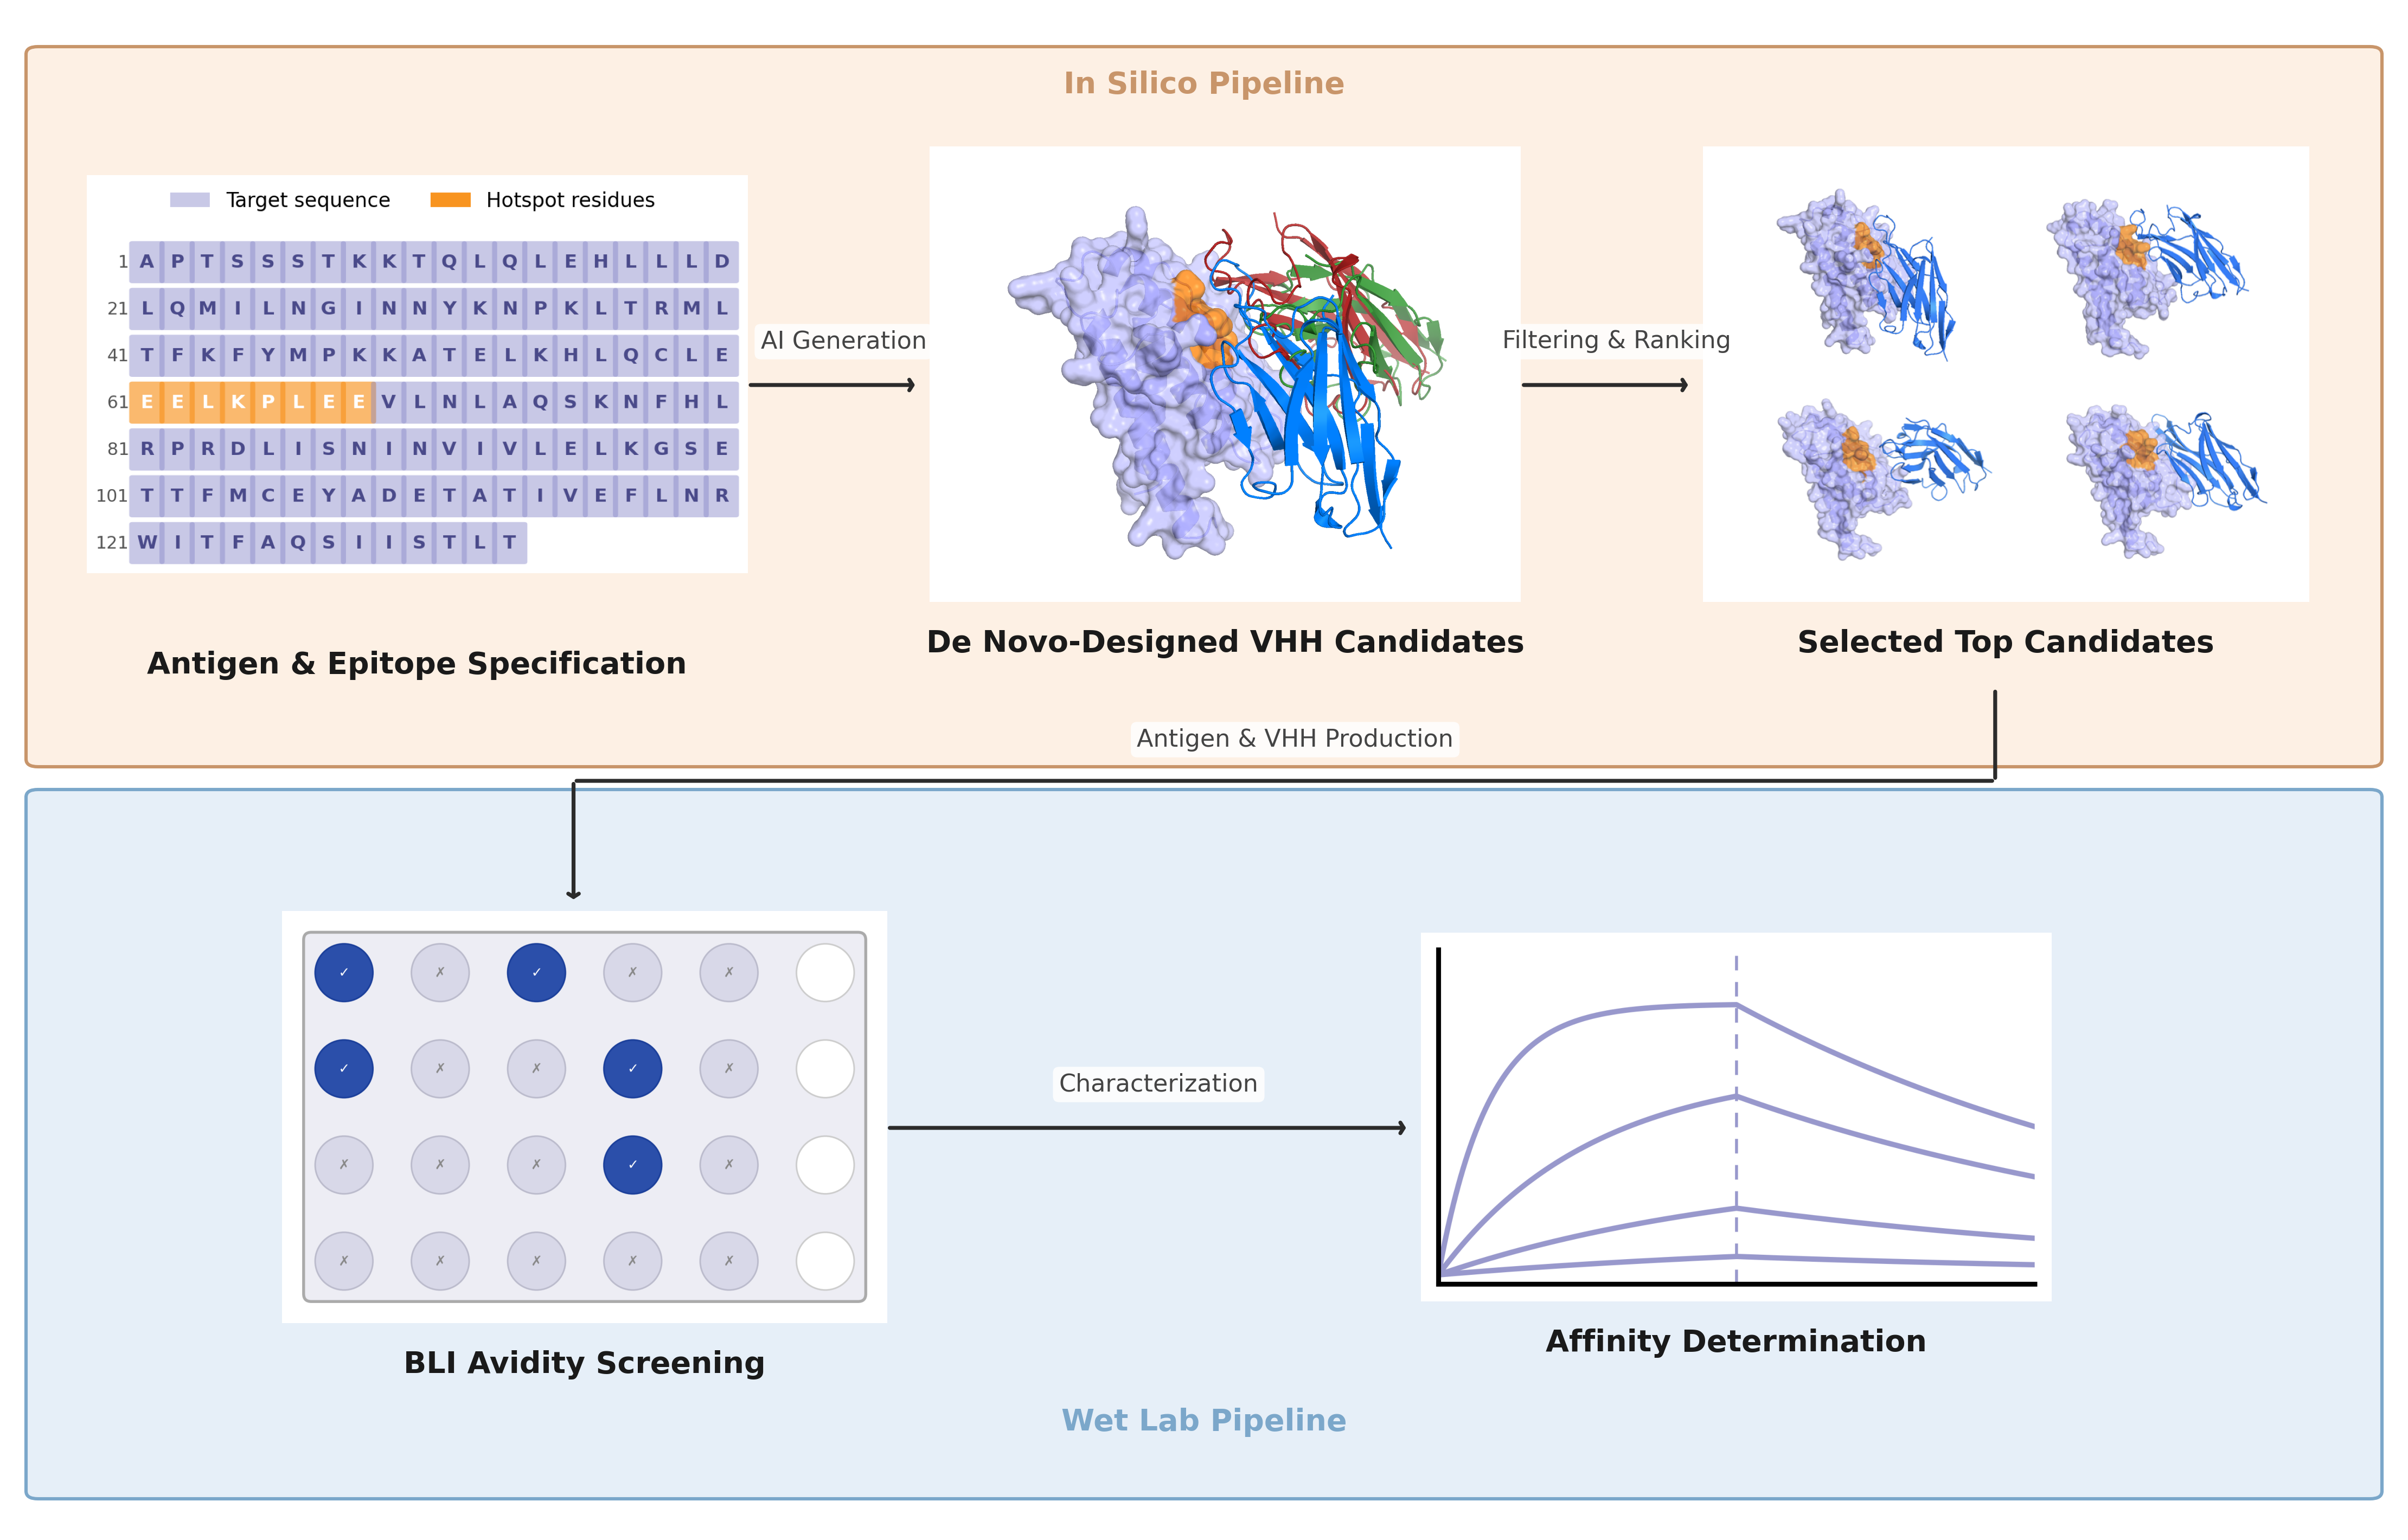
\includegraphics[width=\textwidth]{fig8.png}
  \caption{The MMDesign biologics discovery workflow. Candidate VHH sequences and structures
are generated via hallucination-based optimization (Design), passed through multi-tier computational filtering (Filter), validated by BLI binding assays (Experiment), and characterized by kinetic
analysis (Analyze).}
  \label{fig:workflow}
\end{figure}

\subsection{Target Preparation}
Each campaign requires only an antigen sequence and a set of epitope hotspot residue positions. VHH
scaffold template and CDR loop lengths can be user-specified or automatically assigned.

\subsection{Sequence--Structure Generation}
The generative core operates in a hallucination paradigm: given the antigen sequence, hotspot positions,
and VHH scaffold, the CDR sequences are optimized through backpropagation of customized loss functions
through both the structure-prediction model and a protein language model. These losses encode design
objectives including epitope contact, interface quality, structural plausibility, and sequence naturalness,
guiding the sequence toward regions of the confidence landscape that correspond to high-quality predicted
complexes. Framework regions remain fixed throughout the optimization. Each campaign produces tens of
thousands of candidate VHH sequences.

\subsection{Computational filtering}
The filtering cascade evaluates three successive criteria, each targeting a distinct failure mode:

\textbf{Structural reliability.} Reliability is assessed along four complementary axes: (a) confidence metrics from
a single structure predictor (e.g.\ pLDDT, ipTM), (b) reproducibility across multiple random seeds of the same
model, (c) concordance between two or more independent prediction architectures, and (d) epitope contact
verification: in the predicted complex structure, CDR residues are checked to confirm direct contact with the
specified hotspot positions. Designs that yield divergent conformations under seed or model perturbation
are deprioritized.

\textbf{Expressibility.} A protein language model evaluates sequence naturalness, and a surface-property filter
removes designs with elevated aggregation propensity.

\textbf{Binding specificity.} An in-house developed physics-based scoring function estimates binding free energy
and evaluates whether the predicted interface exhibits features consistent with specific molecular recognition.

After all three tiers, the initial pool of tens of thousands is narrowed to tens of designs for wet-lab testing.
When the number of candidates passing all filters exceeds the experimental budget, the same scoring function
is used to rank and prioritize the final selection.

\subsection{Experimental Characterization}
\textbf{Protein expression and purification.} The CH2 and CH3 sequence of human IgG1 was fused to the
C-terminus of each designed VHH. VHH-Fc constructs were expressed in a CHO system at 10~mL scale for
5 days; supernatant was collected and purified using Protein A magnetic beads. Purity was confirmed by
SDS-PAGE under reducing conditions and SEC-HPLC.

\textbf{Binding characterization.} Multi-cycle kinetic assays were conducted by bio-layer interferometry (BLI)
using a Gator Pivot instrument.

\textbf{Primary binding hit screen.} Target proteins and HSA, each carrying a His tag, were immobilized on
separate NTA biosensors, and VHHs were applied as analyte at a single high concentration (2,000~nM).
Candidates exhibiting binding to the target but not to HSA were classified as specific binders. The assay
sequence was: 60~s baseline 1, 120~s loading (target shift 0.5~nm), 120~s baseline 2, 180~s association phase, 300~s
dissociation phase, and 30~s regeneration and neutralization.

\textbf{$K_D$ determination.} Hits from the primary screen were advanced to quantitative affinity measurement.
VHHs were immobilized on HFC II biosensors via human IgG1 Fc tag, and target proteins were applied
as analyte in four- to seven-point series of two-fold dilutions, enabling accurate kinetic fitting. The assay
sequence was: 60~s baseline 1, 120~s loading (target shift 1.5~nm), 120~s baseline 2, 180~s association phase, 300~s
dissociation phase, and 30~s regeneration and neutralization.

\textbf{General conditions.} All steps were performed at 25~$^{\circ}$C with 10~mM HEPES, 150~mM NaCl, 3~mM EDTA,
and 0.05\% surfactant P20 (pH 7.4) as running buffer. Negative controls (buffer-only samples) were included
for baseline subtraction. Data were collected at 10~Hz and fit globally to a 1:1 binding model across all
concentrations to obtain $K_D$.

\textbf{Poly-reactivity assessment.} To confirm that binding was mediated by specific epitope interactions rather
than non-specific electrostatic interactions, a poly-reactivity ELISA was performed using insulin and dsDNA
as surrogate antigens, coated at 3~$\mu$g/ml at 4~$^{\circ}$C overnight. After blocking with 2\% BSA, VHHs were tested
at two concentrations (5~$\mu$g/ml and 0.5~$\mu$g/ml) and incubated at 37~$^{\circ}$C for 1~h. Detection was performed
with HRP-conjugated anti-human IgG Fc antibody (1:5000), TMB substrate, and 2~M H$_2$SO$_4$ stop solution;
absorbance was read at 450~nm.

\end{document}
